\documentclass[12pt,a4paper]{book}
\usepackage[utf8]{inputenc}
\usepackage[babel, german=quotes]{csquotes}
\usepackage[ngerman]{babel}
\usepackage[T1]{fontenc}
\usepackage{amsmath}
\usepackage{svg}
\usepackage{amsfonts}
\usepackage{amssymb}
\usepackage{mathptmx} % Times
\usepackage{courier}
\usepackage{color}
\usepackage{listings}
\usepackage{nameref}
\usepackage{hyphenat}
\usepackage[left=4cm,right=2cm,top=3cm,bottom=3cm]{geometry}
\usepackage[onehalfspacing]{setspace}
\usepackage[
backend=biber,
style=numeric,
citestyle=authortitle,
sorting=ynt
]{biblatex}
\usepackage{footnote}
\addbibresource{literature.bib}

\definecolor{codegreen}{rgb}{0,0.6,0}
\definecolor{codegray}{rgb}{0.5,0.5,0.5}
\definecolor{codepurple}{rgb}{0.58,0,0.82}
\definecolor{backcolor}{rgb}{0.95,0.95,0.92}

\lstset{
    basicstyle=\ttfamily,
    backgroundcolor=\color{backcolor},   
    commentstyle=\color{codegreen},
    keywordstyle=\color{blue},
    numberstyle=\tiny\color{codegray},
    stringstyle=\color{codepurple},
    breakatwhitespace=false,         
    breaklines=true,                 
    captionpos=b,                    
    keepspaces=true,                 
    numbers=left,                    
    numbersep=5pt,                  
    showspaces=false,                
    showstringspaces=false,
    showtabs=false,                  
    tabsize=2,
}

\author{Falk Gräser}

\title{Entwicklung von Visualisierungs- und Integrationsansätzen für Continuous-Integration und Feature-Branches} 

\includeonly{
	content/1-Abstract,
	content/2-Problemanalyse,
	content/3-Visualiserung-und-Methodiken,
	content/4-Zusammenfassung
}

\begin{document}
\frontmatter

\maketitle

\tableofcontents
\mainmatter
\chapter{Einleitung}

Continuous-Integration ist, spätestens seit der Veröffentlichung \glqq Extreme Programming Explained\grqq{}  von Kent Beck im Jahre 1999,
eine anerkannte Basis für hochqualitative Softwareentwicklung. Knapp 20 Jahre nach dem Werk von Kent Beck ist Continuous-Integration weit
verbreitet und wird vollautomatisiert für Continuous-Deployment genutzt.

Kern von Continuous-Integration ist das kontinuierliche Zusammenführen aller Änderungen, die von Softwareentwicklern eingebracht werden. Continuous-Integration fordert und fördert die Integration dieser Änderungen.
Allerdings fordert gerade diese andauernde und nicht zu umgehende Integration, ein hohes Maß an Kommunikation und erfahrene Softwareentwickler.

Die Anforderung \glqq wann immer der automatische Software-Build fehlschlägt, muss das gesamte Team mit allem stoppen und das Problem sofort beheben\grqq{}\footcite[vgl.][]{humble2010} ist einer der Kernpunkte von Continuous-Integration. Wird das Problem nicht behoben, ist das ganze Team blockiert. Im ungünstigeren Fall werden weiterhin Änderungen zu einem bereits fehlschlagendem Problem hinzugefügt und die Behebung wird zunehmend komplizierter.

Mit dem Erstarken von dezentralen Versionsverwaltungssystemen gibt es eine Alternative zur stetigen Integration. Für jede Anforderung konnte nun mit geringem Aufwand ein eigener Arbeitszweig erstellt werden. Dieser Arbeitszweig wird einzeln entwickelt, getestet und nur im Falle eines positiven Testergebnisses, wieder in den Hauptzweig integriert. Üblicherweise wird für jedes Feature ein solcher Branch erstellt.

Während viele Softwareentwickler dies als kompetente Lösungsstrategie erachten\footcite{ci-is-dead}, sprach sich Martin Fowler im Jahr 2009 intensiv gegen das Feature-Branch-Modell aus\footcite{fowler-feature-branch}.

Während viele moderne und professionelle Lösungen Verfahren für Feature-Branches adaptiert haben und zahlreiche Werkzeuge zur Unterstützung anbieten, gibt es immer noch deutliche Schwierigkeiten. Häufig entwickeln sich \glqq kurzlebige und kleine\grqq{}
Entwicklungszweige zu \glqq großen und langlebigen\grqq{} Veränderungen. Diese betreffen schnell verschiedene Komponenten der Softwareanwendung und werden immer schwieriger zu integrieren.

\section{Zielstellung}

Ziel der Arbeit ist es den Konflikt von \glqq Feature-Branches\grqq{} und \glqq Continuous-Integration\grqq{} aufzuarbeiten, sowie visuelle und methodische Lösungsansätze anzubieten. 

Dazu werden zunächst die Grundlagen und die beiden Begrifflichkeiten selbst erläutert. Es wird auf die automatische Erstellung von lauffähiger Software aus Softwarequellen eingegangen. Die Validierung durch Tests und die Einschätzung der Software durch Software-Metriken wird betrachtet. Schließlich werden Methodiken und Visualisierungen erläutert, welche die beiden vermeintlich konträren Entwicklungsmethoden näher zusammenbringt.

Die Masterarbeit soll sich mit folgenden Thesen auseinander setzen:
\begin{itemize}
\item \glqq Feature-Branches und Continuous-Integration sind unvereinbare Prinzipien.\grqq{},
\item \glqq Continuous-Delivery ist zu komplex, um es in jedem Projekt zu verwenden.\grqq{} und
\item \glqq Der Einsatz von Continuous-Delivery steigert die Qualität des Entwicklungsprozesses.\grqq{}
\end{itemize}
Dabei sollen Indizien oder sogar Beweise jeweils für deren Bestätigung bzw. Falsifizierung geliefert werden.

Weiter werden die Ergebnisse eine Umfrage zu \glqq Nutzungsverhalten von Versionsverwaltungssystemen und Tests\grqq{} erläutert. Die Ergebnisse sollen das Nutzungsverhalten von Versionsverwaltungssystemen und Tests aufzeigen. Als Basis für sowohl Continuous-Integration, als Feature-Branches, können die Ergebnisse der Umfrage eine weitere Perspektive zur Problemstellung beitragen. Schließlich werden anhand eines Prototyp Ansätze für die entwickelten und gesammelten Methoden aufzeigt.

\section{Abgrenzung}

Continuous-Integration und Feature-Branches haben einen starken Einfluss auf den Software-Entwicklungsprozess in dem sie angewendet werden. Daher existieren unter anderem Schnittmengen zu den Themenbereichen Anforderungsmanagement, Psychologie und \\Continuous-Deployment. 
Da der Fokus der Arbeit auf dem Konflikt der beiden Methodiken liegt, werden die benannten Bereiche nur angeschnitten. Das Anforderungsmanagement und die psychologische Komponente sind beide notwendig, für die Durchführung von Continuous-Integration und Feature-Branches. Allerdings üben weder das Anforderungsmanagement, noch psychologische Einflussfaktoren eine deutlichen Einfluss auf den Konflikt zwischen Continuous-Integration und Feature-Branches aus. 

Continuous-Deployment würde ebenso den Rahmen der Betrachtung überschreiten. Continuous-Deployment-Prinzipien greifen primär, nachdem Änderungen von Entwicklern integriert wurden. Als Teilaspekt von Continuous-Deployment, wird Continuous-Delivery stärker beleuchtet.

\chapter{Problemanalyse}

Die Zusammenführung der Arbeit von mehr als einem Entwickler ist ein komplexer und nicht trivialer Vorgang. \\
Viele Teile eines Softwareprojektes beeinflussen andere und häufig werden an Schnittstellen in Programmen Änderungen von mehreren Entwicklern vorgenommen. \\
Es muss sichergestellt werden, dass die Änderungen zusammengeführt werden können und dass das Ergebnis syntaktisch und semantisch korrekt ist, sowie den Anforderungen entspricht.

Während die syntaktische und semantische Validierung klassische Themen der theoretischen Informatik sind, erfordert die Erhebung und Aufbereitung von Anforderungen eine ganz eigene Betrachtung durch ein konkretes Anforderungsmanagement.

Gerade wenn die Software einen gewissen Umfang übersteigt, ist daher ein solides Anforderungsmanagement essenziell. Zudem müssen Mechanismen geschaffen werden, um sicherzustellen, dass diese Anforderungen über die komplette Laufzeit der Software erfüllt bleiben. 

Leider sieht die Realität in der Softwareentwicklung nicht selten anders aus. Fehlende, nicht dokumentierte oder veraltet Anforderungen sind keine Seltenheit.\\
Ebenso sind lange Zeitintervalle in denen sich Teile der Software in keinem lauffähigen oder einem fehlerbehaftetem Zustand befinden häufig anzutreffen.

Fehlende Anforderungen und fehlerhafte Umsetzungen werden häufig erst zum Zeitpunkt des Testes - oder schlimmer - zum Zeitpunkt der Auslieferung offenbart.

Die Gründe für diese Schwierigkeiten sind häufig in kein homogenes Bild zu bringen. Vielmehr tragen verschiedene Faktoren dazu bei, die erst in der Kombination zu erheblichen Problemen führen können.

\section{Vorgehensmodelle}

Um komplexe Software in einer strukturierten und definierten Herangehensweise zu erstellen, wurden ausführlich beschriebene und wohl definierte Vorgehensmodelle definiert. Ziel war eine klare Schrittfolge mit eindeutigen Zielstellung, wie man es aus anderen Ingenieursdisziplinen gewohnt war. 

Die daraus entstehenden Modell hielten sich meist an eine klare Folge aus Planungsphase,  Konzeptions-, Implementierungs-, Test- und Abnahmephase. Beispiele sind hier das Wasserfallmodell und das V-Modell. Gerade in bereichen höchster Sicherheit und einer starken Bindung an bürokratische Strukturen wird auch heute noch das V-Modell erfolgreich eingesetzt[quote Referenz Bund?].

Mit der komplexität einer Software steigt in der Regel auch der Umsetzungsaufwand und die damit verbunden Zeit. Durch die klare Phasenteilung in den klassischen Vorgehensmodellen, kann daher von der Anforderungsaufnahme bis zu Auslieferung einiges an Zeit verstreichen. Nicht selten ändern sich allerdings Anwendungsszenarien und Benutzeranforderungen an das entstehende System. Eine weitere Schwierigkeit ist die Prüfung der Umsetzung von Anforderungen. Sollte die Umsetzung einer Anforderung, zum Beispiel durch ungenaue oder mehrdeutige Angaben, nicht den Maßgaben des Tests entsprechen, vergehen Wochen oder Monate bis diese Diskrepanz aufgedeckt wird.

Immer wieder kam es daher zu unbefriedigenden oder sogar gescheiterten Softwareprojekten. Gerade bei komplexen Softwaresystem mit einem entsprechenden Umsetzungsaufwand, ist der Schaden dann sehr hoch.

Um diesen Schaden zu minimieren entwickelte sich eine alternative Herangehensweise, welche vor allem Interaktion, Funktionalität, Kundenorientierung und Veränderungsbereitschaft als wichtig erachtet. Festgehalten im Agilen Manifest[quote manifest] proklamierten viele bekannte und angesehene Softwareexperten ihren Willen Softwareprojekte grundsätzlich anders zu fokussieren.

Beeinflusst von der Lean-Bewegung aus der Automobil-Fertigungsindustrie\footcite{kent1999} wollte man die Produktivität deutlich steigern und aus den bürokratisch anmutenden Vorgehensmodellen ausbrechen.

Das Agile Manifest stellt hohe Ansprüche an Entwickler und erzwingt ein Umdenken im Umgang mit dem Projektprozess. Während in traditionellen Vorgehensmodellen jede Phase eine längere zeitliche Periode einnimmt, so werden diese Phasen und Zeiträume in agilen Vorgehen deutlich verkürzt, um damit einhergehende Informationsflüsse deutlich zu beschleunigen.
Diese kurzen Zeiträume und damit einhergehenden vielen Iterationen geben kontinuierlich und schnell Auskunft über den Zustand eines Projektes. Außerdem wird es einfacher zu erkennen, welche Schritte tatsächlich wertvoll sind und welche Schritte dem Projektfortschritt eher abträglich sind. 

Oberstes Ziel hierbei ist die Lieferung von ``wertvoller'' Software, also die Einschätzung der Anforderungen mit den Stakeholdern und priorisierte Lieferung dieser Anforderungen.

Dieses Vorgehen führt automatisch dazu, dass frühzeitig deutlich wird, ob die richtigen Anforderungen als wichtig erkannt wurden und welche Anforderungen implizit angenommen und daher im verborgenen lagen.

Ein weiterer Aspekt ``wertvoller'' Software ist ihre Funktionalität. Diese sicherzustellen in einer kontinuierlichen Auslieferung erfordert ein hohes Maß an Qualitätssicherung. Schon sehr früh im Entwicklungsprozess eines iterativ wachsenden Systems wird deutlich, dass keine menschliche Resource mehr im Stande ist, alle Anforderungen mit jeder Auslieferung zu testen und die Qualität sicherzustellen. Die Automatisierung dieser Tests ist somit unausweichlich.

\section{Qualitätssicherung und Softwaretest}

Die Qualitätssicherung einer Software muss als oberste Prämisse sicherstellen, dass alle Anforderungen erfüllt sind und dass die Anforderungen auch erfüllt bleiben. Nicht selten führen Neuerungen in einer Software dazu, dass bereits bestehenden Funktionalität beeinträchtigt wird. 
Aufbauend auf der Annahme, dass alle notwendigen Anforderungen beschrieben sind, müssen diese in unterschiedlichen Ebenen überprüft und sichergestellt werden.
Diese Ebenen richten sich danach welche Anforderungen und damit verbundenen Merkmale geprüft werden müssen, aber auch danach wie komplex die damit verbundene Prüfung ist.

In der Literatur werden meist Unit-, Funktions- und Integrationstests, sowie System- und Abnahmetests (Akzeptanztest) unterschieden.
Die Unterscheidung liegt hier in der Größe des zu betrachtenden Ausschnitts der Software und damit der zu prüfenden Aussage. Während in einem Abnahmetest eine direkt Verbindung zwischen Anforderung und Testfall hergestellt werden kann, so ist dies in einem einzelnen Unittest meist nicht mehr möglich.
\paragraph{Akzeptanztest}
Akzeptanz- oder auch Abnahmetests stellen in erster Linie die Erfüllung der definierten Anforderungen sicher. Akzeptanztests werden häufig in der Form von Anwendungsszenarien (Use-Cases) beschrieben und sollte sicher daher nur auf das Zusammenspiel von Systemen und Akteuren beziehen. Die Verwendung von technische Details der Software, wie Datenbankspezifikationen oder konkrete Systemimplementierungen sollten vermieden werden. Nicht nur erhöht es den Wartungsaufwand dieser Tests, es verschiebt auch den Fokus des Tests weg von den eigentlich zu prüfenden Merkmalen und Aktionen.

Nicht notwendiger Weise, aber häufig dauert die Durchführung der Akzeptanztests recht lange. Daher werden sie meist seltener ausgeführt. Die lange Ausführungszeit macht sie zudem unhandlich, um eine schnelle Validierung eines in Entwicklung befindlichen Softwarestückes zu gewährleisten.

\paragraph{Funktions- und Integrationstests}

Funktions- und Integrationstests dienen der Überprüfung von Schnittstellen. Es wird sichergestellt, dass verschiedenen Teile der Software, verschiedene Komponenten, nach den vereinbarten Schnittstellen miteinander kommunizieren.
Neben der Absicherung von Seiteneffekten zu anderen Komponenten und Fremdmodulen, bieten Integrationstests auch eine gute Beschreibung einer Komponente und derer Schnittstellen.

\paragraph{Unittests}

Unittests bilden die unterste Ebene der Softwaretests. Maßgeblich bei Unittests ist die völlige Abkopplung von anderen Teilen, als des zu testenden Teils (Unit) der Software. Jegliche Interaktion mit externen Services sollte strikt vermieden werden.
Ein ordnungsgemäß verfasster Unittest stellt neben der Regressionssicherheit eines Moduls auch einen Teil dessen Dokumentation sicher. Da ein Unittest das zu testende Modul initialisiert und die notwendigen Schnittstellen bereitstellt, bildet er auch anschaulich die Intention des Moduls ab.

\section{Automatisierung der Softwareerstellung}

Die Bereitstellung einer Software baut auf mehreren Faktoren auf. Es wird ein konkreter Stand der Softwarequellen benötigt, ein ausführendes System und es muss für eine Übersetzung der Softwarequellen zu dem System gesorgt werden.
Je nach Anforderung der Software und des Ausführungsszenarios reicht dieser Vorgang von einer trivialen Kopie zu einem mehrstufigen, komplexen Vorgang. 

Im nachfolgenden wird beschrieben wie Software in einen wohldefinierten, funktionalen Zustand gebracht und dieser validiert wird. Dazu wird auf Versionsverwaltungssysteme, Konfigurationsmanagement, die automatisierte Erstellung und deren Test eingegangen.

\subsection{Kodeverwaltung und Versionsverwaltungssysteme}

Bereits frühzeitig wurde in der Bereitstellung von Software in Programmversionen unterschieden. Anwender konnte so transparent nachvollziehen, wie fortschrittlich die Anwendung war, die sie erwerben wollten.
Für die Entwicklung ergab sich daraus vor allem die Herausforderung nachfolgende Fehlerkorrekturen für viele verschiedene Entwicklungszustände bereit zustellen.
Eine nachvollziehbare und wartungsarme Ablage der einzelnen Versionsstände war daher unabdingbar.

Auch wenn es möglich ist alle Programmversionen in manuell gepflegten Ablagen zu verwalten, gelangt die Entwicklung einer komplexen Software schnell an den Punkt an dem eine Ablage zusätzliche Bedingungen erfüllen muss.

Das dabei herausstechende Merkmal ist die Zustandssicherheit. Es muss gewährleistet sein, dass der Quellcode für eine bestimmte Version in einem konkreten, definierten Zustand ist. Als weiteres Merkmal ist die Transparenz anzuführen. Transparenz ist vor allem dann von Nöten, wenn mehr als ein Entwickler an einer Quellcodesammlung arbeitet. Schnell geht die Übersicht verloren, welche Änderungen wann, von wem und warum eingebracht wurden. Oftmals sind diese Informationen aber hilfreich um Entscheidungen im Entwicklungsprozess zu treffen.

Über die Entstehung von Versionsverwaltungssysteme[quote Soft.Quali] haben sich vor allem zwei Prinzipien herausgebildet: Zentrale und Dezentrale Versionsverwaltungssysteme. Zwar unterscheiden sich die Versionsverwaltungssysteme auch in anderen Merkmalen, zum Beispiel in der Ablage der Quellen und deren Änderungen, diese Merkmale haben aber nahezu keinen Einfluss auf die Verwendung im Softwareentwicklungsprozess.

Auch wenn heutzutage die dezentralen Versionsverwaltungssystem stark zunehmen, so fällt bei näherer Betrachtung auf, dass diese oft primär als zentrale Versionsverwaltungssysteme verwendet werden.

\paragraph{Zentrale Versionsverwaltungssysteme} folgen dem Prinzip, dass es nur einen zentralen Punkt gibt auf dem alle Versionstände gespeichert werden. Dieses ``single point of truth'' Prinzip sorgt für einen einfachen Kontrollfluss, welcher dafür sorgt, dass alle Partizipierer mit einfachen Mitteln auf den gleichen Versionsständen arbeiten. Damit einhergehend ist eine Übersicht aller Änderungen problemlos möglich.

Nachteil dieser Variante ist häufig der Initialaufwand, da eine zentrale Komponenten bereitgestellt werden muss. Zudem sind zentrale Systeme generell störanfälliger und Probleme betreffen immer alle Teilnehmer gleichzeitig.
Je nach verwendeter Versionierungsstrategie kann es zudem zu einer zentralen Blockade ganzer Bereiche der Softwarequellen kommen, wenn diese für eine exklusive Bearbeitung gesperrt sind.

\paragraph{Dezentrale Versionsverwaltungssysteme} benötigen im Gegensatz keine zentrale Instanz und können problemlos in einem losen Verbund von Einzelsystemen betrieben werden. 
Im Gegensatz zur zentralen Verwendung, existierend dadurch deutlich mehr Zustände, die ohne entsprechende Maßnahmen nicht zu überblicken sind. Dieser Mehraufwand bringt allerdings eine Flexibilität mit sich, welche viele Möglichkeiten bietet um Softwareänderungen zu koordinieren. Änderungen können in ihrer Reihenfolge transparent manipuliert und der Zeitpunkt der Zusammenführung beliebig gewählt werden. 
Im Bereich ``Feature Branches'' werden Versionierungsstrategien im Detail erläutert.

Ihrer dezentralen Natur geschuldet, sind sie ausfallsicherer als die zentralen Versionsverwaltungssysteme, benötigen allerdings die entsprechenden Informationen und Befugnisse zur Verbindung, um diesen Vorteil nutzen zu können.

\subsection{Konfigurationsverwaltung}
\label{subsec:konfigurationsverwaltung}

Konfigurationsverwaltung ist eine wichtige Basis für die automatisierte Erstellung eines Softwareprojektes. Sie definiert wie alle Artefakte in einem Softwareprojekt orchestriert werden. Im Detail wird dabei Erstellung, Identifikation, Validierung und Ablage geregelt. Neben den Projekteigenen Artefakten müssen aber auch deren Umgebung genau definiert sein. \footcite{humble2010}

Ein lockerer Umgang mit der Konfigurationsverwaltung kann gerade zu Anfangs ohne nennenswerte Folgen einhergehen. Spätestens aber während der Reifung und Alterung eines Softwareprojektes sind Folgen deutlich zu spüren. Gerade wenn sich unbemerkt die Version oder Konfiguration der Software eines Drittanbieters ändert, kann dies zu sehr schwer zu identifizierbaren Problemen führen. In anderen Fällen reicht es allerdings auch, wenn sich die Konfiguration zwischen Entwicklungs- und Produktivumgebung leicht unterscheidet. Auch hier können damit zusammenhängende Fehler unnötig viel Zeit in Anspruch nehmen.

Im Idealfall kann eine vollständige Konfigurationsverwaltung:
\begin{itemize}
\item eine Umgebung bereitstellen, die genau definiert welches Betriebssystem, in welcher Version, installiert ist und welche Anwendungen, mit welcher Konfiguration, darauf liegen
\item auf jeder Umgebung jeden dieser Bestandteile einzeln inkrementell verändern und diese Änderungen auch synchronisiert bereit stellen.
\item alle Änderungen mit Zeitpunkt und Verursacher einfach darstellen
\item Sicherheitsregeln und Konventionen über alle Systeme sicherstellen
\item alle diese Funktionalitäten barrierefrei dem Entwicklungsteam zur Verfügung stellen
\end{itemize}

Alle Forderungen sind sicherlich nicht immer Notwendig, sorgen aber dafür, dass Projekte langfristig, mit geringem Aufwand betreut werden können. Zudem wird deutlich, dass Virtualisierung und Versionsverwaltung[quote cont.deliv] der entsprechenden Komponenten den einhergehenden Aufwand deutlich verringern können.

\subsection{Abhängigkeitsverwaltung}

In der Abhängigkeitsverwaltung werden die Softwareabhängigkeiten der Anwendung beschrieben. In auf  Komponenten basierenden Anwendungen schließt dies die eigenen, interne Abhängigkeiten mit ein. Diese Abhängigkeiten, meist Module genannt, sollen die mit monolithischen Strukturen einhergehenden Nachteile unterbinden. Monolithen leiden häufig unter einer schwachen Softwarearchitektur und entwickeln sich daher entsprechend schlecht weiter. Mögliche Skalierungen des Systems oder ein Austausch von einzelnen Bestandteilen sind mit einem erheblichen Mehraufwand verbunden.

Ist eine Anwendung hingehen auf mehrere Komponenten aufgeteilt, kommen neben den genannten Vorteilen der Skalierbarkeit und Austauschbarkeit, auch Vorteile für das verteilte Arbeiten von Teams. Allerdings führt eine Komponenten basierende Anwendung natürlich auch zu einem organisatorischem Mehraufwand. Dieser Mehraufwand besteht in der Beschreibung der Abhängigkeiten und der Auflösung des damit entstehenden Abhängigkeitsgeflechtes. Übliche Abhängigkeitsverwaltungen verwenden hierzu Versionsnummer aus der Versionsverwaltung, sowie eine Paketbeschreibung in einem eigenen Format. 

Für die automatisierte Erstellung der Softwareanwendung ist es erforderlich, ähnlich wie bereits bei der Versionsverwaltung, ein eindeutiges Abhängigkeitsbild zu beschreiben. Während zum Auflösen der Abhängigkeiten meist mehrdeutige Ausdrücke verwendet werden, die eine Bandbreite an Versionen der Abhängigkeiten erlauben, ist für den Erstellungsvorgang wichtig die konkret verwendeten Versionen zu dokumentieren und mit dem erstellten Produkt auszuliefern. Ähnlich der erwähnten Paketbeschreibung, wird dies mit einer Lock-Datei gesichert.

\subsection{Automatisierte Erstellung und Auslieferung}

Der an sich triviale Schritt, der Erstellung (Build) einer Anwendung, birgt gewisse Tücken. So kann die Ausführung eines komplexen Erstellungsskriptes einen sehr langen Zeitraum in Anspruch nehmen und ein besonders kompliziertes Skript kann die Arbeit damit intransparent gestalten und das Entwicklungsverhalten deutlich benachteiligen. [quote paper] Werden bei einem Erstellungsskript Aspekte der vorangegangen Abschnitte zu Versions-, Konfigurations- und Abhängigkeitsverwaltung nicht berücksichtigt, können zudem inkonsistente und damit nicht wiederholbare Resultate erzeugt werden. Diese können leicht zu schwer oder nicht auffindbaren Fehlern führen.

Ziel bei der Erstellung eines Erstellungsskriptes ist es folglich einen konsistenten und transparenten Ablauf zu befolgen. Dies wird unter anderem durch die korrekte Versionsverwaltung der einzelnen Komponenten, Konfigurationen und Abhängigkeiten erreicht. Mit diesen Informationen können erstellte Produkte, auch ``build artifacts'' oder Artefakte genannt, in einem zentralen Artefakt-Lager abgelegt werden. Dies gewährleistet sowohl einen schnellen Zugriff auf Teilartefakte, als auch einen konsistentes Ergebnis bei der Erstellung der Auslieferung.

Die Auslieferung der Software ist direkt mit der Erstellung verwoben. Bei jeder Auslieferung muss sichergestellt werden, dass Software auf dem entsprechenden Zielsystem auch lauffähig ist und dass sie richtig konfiguriert ist für das Zielsystem. Ein vollständiges Konfigurationsmanagement beschreibt die Systemabhängigkeiten und sorgt folglich für die korrekte Auslieferung der richtigen Artefakte.

Sowohl bei der Erstellung, als auch bei der Auslieferung ist insbesondere auf eine vollständige Beschreibung und die Einhaltung dieser zu achten. Gerade auf Entwicklungssystemen können Abhängigkeiten vorhanden sein, welche zwar für die Funktionalität der Anwendung sorgen, allerdings nicht beschrieben wurden. Bei der Auslieferung auf andere Systeme können diese ``Schattenabhängigkeiten'' dann zu erwartetem Verhalten oder Abstürzen führen. Ein sehr kontrollierter Ausweg aus dem Dilemma von mehrfach genutzten Entwicklungsumgebungen bietet die Virtualisierung der verwendeten Systeme. Wie bereits für Softwareabhängigkeiten der Anwendung beschrieben, können diese Virtualisierungen als Artefakte bereitgestellt werden und unterstützen Konsistenz, Transparenz sowie Skalierbarkeit[quote virtualiserung mit docker].

Bei der Auslieferung der Software können grob zwei Stufen der Automatisierung unterschieden werden. Eine Stufe ist die manuell angestoßene Auslieferung, bei der der Zeitpunkt der Auslieferung davon bestimmt wird, wann das automatisierte oder automatisiert-moderierte Script ausgeführt wird. Eine Andere ist die vollautomatisierte Auslieferung, bei der der Zeitpunkt lediglich von der Durchlaufzeit einer Änderung durch die Qualitätskontrolle bestimmt wird.
Des weiteren werden unterschiedliche Auslieferungsstrategien (``deployment strategies'') unterschieden, es seien an dieser Stelle nur exemplarisch das ``blue green deployment'' und das ``canary deployment'' genannt. Die Auslieferungsstrategien werden dabei je nach Anforderungen ausgewählt und haben Vorzüge wie Ausfallsicherheit, Bewertung der ausgelieferten Änderung oder Skalierbarkeit der Zielsysteme.

Da die konkrete Auslieferung auf die Bereiche ``Continuous Integration'' und ``Feature Branches'' nur begrenzt Einfluss hat, verweise ich an dieser Stelle auf die entsprechende Fachliteratur.

\subsection{Validierung und Test}

Die Validierung einer Software ist ein unglaublich komplexes Unterfangen. Die vollständige Richtigkeit eines Programmes zu beweisen, scheitert bereits bei kleinen Anwendungen, da die Programmkomplexität schlicht zu schnell steigt. Zudem können nur Teile validiert und getestet werden, welche im Vorfeld bestimmt worden sind. Unklare, mehrdeutige oder fehlende Anforderung machen einen Test unvollständig oder nehmen im die Aussagekraft[quote software quali p243 kap4.6].

Da eine Software nicht vollständig getestet werden kann, muss eine Strategie gewählt werden, welche Tests verwendet werden und mit welchem Ziel. Zudem können Metriken gewählt werden, die eine Aussage über die Testvollständigkeit liefern können. Bei der Entscheidung welche Strategie gewählt wird, fallen verschiedene Kriterien ins Gewicht. Zum einen muss betrachtet werden, welche Anforderungen mit welchem Testverfahren getestet werden können, zum anderen welche Granularität für jeden Test verwendet wird.

Insbesondere in der automatisierten Erstellung sind diese Entscheidungen wichtig, da sie eine Basis liefern für die Aussage, wie schnell die Testsammlung ausgeführt werden kann. Und damit einhergehend, wie schnell kann eine Aussage getroffen werden, ob ein Inkrement der Software valide ist. 
Ein wichtiger Punkt ist hier auch die aktive Wartung der Testsammlung, jeder Fehler der nicht von der Testsammlung erfasst wurde, muss spätestens nach der Beseitigung des Fehlers auch durch die Testsammlung validiert werden. Diese Regressions-Sicherheit stellt in vielen Testsammlungen häufig den größten Teil der Tests [quote software quali].

Da Tests und Metriken die einzigen Möglichkeiten sind um automatisch Einschätzungen der Software vorzunehmen, werden diese Bereiche erneut im Kapitel~\ref{ch:visu_meth} aufgegriffen und näher auf deren Wertschöpfung eingegangen.

\section{Continuous Integration}

Continuous Integration wurde sehr treffend beschrieben \footcite{fowler2006}
\blockquote {Continuous Integration is a software development practice where members of a team integrate their work frequently, usually each person integrates at least daily - leading to multiple integrations per day. Each integration is verified by an automated build (including test) to detect integration errors as quickly as possible.}

Continuous Integration wurde erstmal von Kent Beck als Teil einer Reihe von Praktiken des Entwicklungsvorgehens ``Extreme Programming''\footcite{kent1999} beschrieben. Die Idee die Integration von Codeständen zu fördern, in dem man die Entwickler anhält ihre Änderungen täglich oder häufiger abzugleichen und durch einen automatisierten Vorgang als lauffähig zu beweisen. Damit konnten Fehler zum Zeitpunkt des Auftretens gefunden werden, insbesondere Fehler, welche erst durch die Integration mit den Änderungen anderer Entwickler auftreten. Damit fordert Continuous Integration zugleich auch eine aussagekräftige Testabdeckung mit automatischen Tests und dass Entwickler einen entdeckten Fehler direkt beheben, da sonst alle anderen Teammitglieder behindert werden.

Die Arbeitsweise alle Änderungen auf einem Zweig zu vereinen und kontinuierlich zu vereinigen, wird auch Trunk-Based-Development genannt. Während Continuous Integration und Trunk-Based-Development als getrennte Methodiken geführt werden\footcite{trunkbaseddevelopment}, so werden sich doch häufig in Kombination oder synonym verwendet\footcite{fowler-feature-branch}.

Natürlich nutzt Continuous Integration auch alle Vorteile, die im Kapitel ``Automatisierung der Softwareerstellung'' beschrieben werden. Modularisierung, Konfigurationsbeschreibung, automatische Erstellung und Wiederverwendbarkeit von Artefakten, sowie eine generelle Strategie, die Software so zu entwickeln, dass sie gut testbar ist. Die vollständige Erfüllung dieser Kriterien fordert und fördert eine gute Entwicklungskultur. Dies ist auch der Grund warum Continuous Integration seit den Beschreibungen von Kent Beck so sehr an Akzeptanz und Bedeutung gewonnen hat.

Während die Vorteile von Continuous Integration sehr deutlich und gewichtig sind, gibt es auch Kosten die mit dieser Technik einhergehen. Die komplette Automatisierung erfordert einen durchaus wahrnehmbaren Aufwand in der initialen Einrichtung und einen häufig unterschätzten Aufwand in der Aufrechterhaltung. Gerade bei weniger wichtigen Projekten oder bei Projekten unter besonders hohem Druck, kann es passieren, dass wichtige Bestandteile von Continuous Integration vernachlässigt werden. Dass heißt die Testabdeckung sinkt deutlich oder etwa Teile des Konfigurationsmanagements werden umgangen und essentielle Abhängigkeiten von Hand gepflegt. Dieses Verhalten widerspricht offensichtlich der langfristigen Wertschöpfung und bricht mit den Prinzipien von Continuous Integration. Leider sind aber menschliche Schwächen auch in Continous Integration noch ein Problem, welches nur durch Training und Motivation zur Selbstdisziplin der Entwickler behoben werden kann. In Kapitel~\ref{ch:visu_meth} wird auch das Thema Entwicklerdisziplin erneut aufgegriffen und auf die Gratwanderung von gesunder Entwicklungskultur und destruktiver ``blaming culture'' eingegangen.

\section{Dezentrale Versionierung mit Git}

Im Kapitel~\ref{subsec:konfigurationsverwaltung} Konfigurationsverwaltung wurde bereits auf das Thema Versionsverwaltung eingegangen. Als das populärste System im Open-Source-Bereiche und eines der großen Systeme im kommerziellen Bereich\footcite{g2crowd2018}, wird nun anhand von Git erläutert, wie die dezentrale Versionsverwaltung grundlegend verwendet wird. Außerdem kommen einige git-spezifische Merkmale hinzu, welche bei der visuellen Aufbereitung wichtig werden.

Git wurde vom Linux-Schöpfer Linus Torwalds im April 2005 initiiert, aus der Not heraus sich vom vorher verwendeten ``BitKeeper''-System zu lösen, da diese nicht mehr mit der eigenen Open-Source-Lizenz in Einklang zubringen war. Git wurde von vornherein als verteiltes, vor Verfälschungen sicheres und effizientes Versionsverwaltungssystem entworfen. Diese Eigenschaften und die Software-Plattform ``GitHub'', machten Git in den letzten 13 Jahren zum de-facto Standard für Versionsverwaltung\footcite{heise-torvald-git2015}.

Als dezentrales Versionsverwaltungssystem ist einer der großen Vorteile von Git, dass die vollständige Historie der Dateien lokal verfügbar ist. Während zentrale Versionsverwaltungssysteme immer einen dedizierten Server benötigen, können dezentrale Varianten über Peer-To-Peer-Schnittstellen kommunizieren. Diese Eigenschaft sorgt neben einer hohen Ausfallsicherheit und Informationsredundanz, auch für eine hohe Flexibilität und die Möglichkeit zahlreiche Arbeitsweisen von Softwareentwicklern zu unterstützen.

\subsection{Definition und Verwendung der Git-Artefakte}

Die Verwendung von git gestaltet sich vergleichsweise einfach. In wenigen Schritten kann Git installiert \footcite{git-scm-install} und mit der Verwendung begonnen werden. 
Git nutzt bestimmte Artefakte um seine Aufgaben zu erfüllen. Darunter Repositories, Commits, Branches und Tags. Zudem werden Mechanismen bereitgestellt um mit diesen Artefakten zu interagieren. Neben zu erwartenden Mechanismen wie Hinzufügen und Löschen, werden auch Speichern- und Ladeaktionen (``push'' und ``pull) angeboten\footcite{git-essentials-2017}.

\begin{figure}[htbp]
  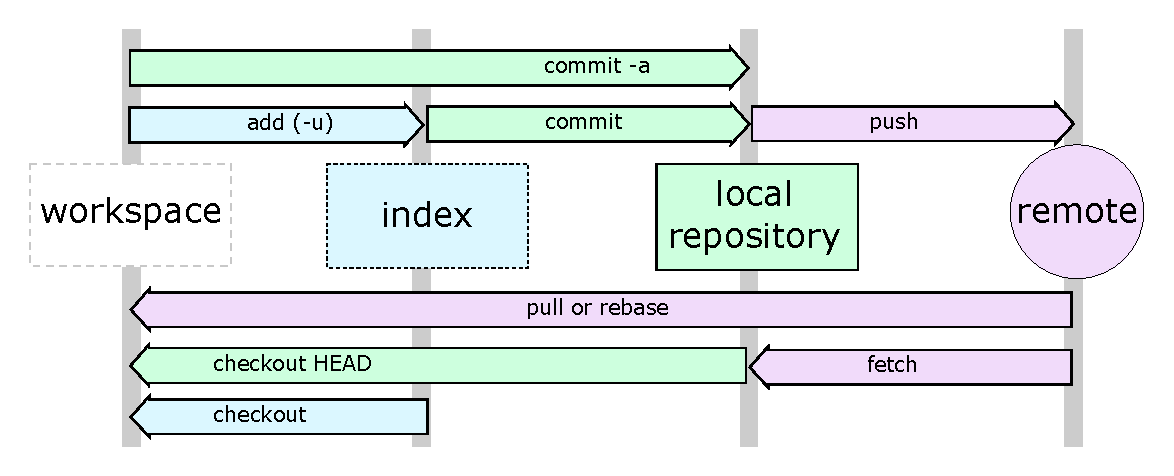
\includegraphics[
    width=\textwidth,
    height=\textheight,
    keepaspectratio
  ]{resources/git-workflow.pdf}
  \caption{Git-Workflow}
  \label{git-workflow}
\end{figure}
Die Grafik~\ref{git-workflow} stellt das Zusammenspiel der Artefakte und den Standard-Git-Worflow\footcite{osteele-git-workflow} dar.

\paragraph{Repositories} sind die größte Verwaltungseinheit in Git. Diese enthalten alle Git-Objekte, wie Referenzen, Commits, Trees, Blobs, sowie die lokale Konfiguration. Repositories können andere Repositories referenzieren oder referenziert werden, dabei können viele gängige Protokolle verwendet werden (http, ssh, ftp, absolute Pfade)

\paragraph{Commits} sind zeitlich determinierte, persönliche und kommentierte Referenzen auf einen konkreten Arbeitsstand (``Snapshot'') des Repositories. Ein Commit kann immer maximal nur auf einen Eltern-Commit verweisen, kann allerdings von beliebig vielen anderen Commits referenziert werden. Bei Betrachtung aller Commits, bilden dieser daher einen gerichteten Baumgraphen.

\paragraph{Branches} sind, im Gegensatz zu vielen anderen Versionverwaltungssystemen, in Git lediglich Verweise auf einen bestimmten Commit. Wenn ein Branch aktiv ist, dann wird mit jedem Commit auf diesem Branch, der Verweis auf den neuen Commit aktualisiert.

\paragraph{Tags} sind genauso wie Branches einfache Verweise auf einen Commit, allerdings verändert sich die Position eines Tags nach einem Commit nicht.

\paragraph{Remotes} sind Verweise in der Konfiguration eines Repositories auf andere Repositories. Dies wird im allgemeinen genutzt um Änderungen von dort zu holen oder dorthin zu bewegen. Es können beliebig viele Remotes für jedes Repository definiert werden. Zudem kann beliebig definiert werden, welche Branches von einem Repository Änderungen erhalten oder dieses aktualisieren.

\paragraph{Blobs} sind die komprimierten Inhalte einer Datei.

\paragraph{Trees} sind Referenzen von Blobs, und stellen damit im einfachsten Fall eine Ansicht eines Verzeichnisses und seiner Dateien dar.

\paragraph{Hashes} sind im allgemeinen Abbildung einer großen Abbildung von Zeichen auf eine deutlich geringere Menge. Die Abbildung führt immer zur gleichen Ergebnismenge. In Git werden Hashes als allgemeine Referenzierungsmöglichkeit verwendet. Alle Relationen werden darüber beschrieben und sind daher über alle Repositories gleich. Um die Eindeutigkeit 

\subsection{Interne Arbeitsweise}

Git verwendet intern einen Mix aus Referenzen, Indexierung, Komprimierung und Hashing. Zudem werden keine Differenzmengen, wie etwa in Subversion abgelegt, sondern immer vollständige Dateiinhalte. Diese Kombination bedeutet für viele Softwareprojekte eine deutliche Speicherplatzreduktion, wie zum Beispiel für das Mozilla-Projekt\footcite{kernel-git-svn}. Dadurch dass vollständig Dateiinhalte gesichert werden, ist Git für besonders große, schlecht zu komprimierende, sich häufig ändernde Dateien eher ungünstig. Für solche Dateien ist es sinnvoller 

Um die interne Arbeitsweise von Git zu erläutern, müssen die Zusammenhänge von Commits, Trees, Blobs und Hashes verdeutlicht werden.

Die Git-Objekte werden von Git immer anhand ihres Hashes abgelegt. Dabei wird ein 40-Stelliger SHA1-Hash verwendet. Die notwendigen Stellen zu Referenzierung sind aber häufig deutlich geringer, so können im allgemeinen Gebrauch deutlich verkürzte Zeichenketten verwendet werden. Im allgemeinen etwa 5 Stellen oder bei großen Projekten, wie dem Linux-Kernel, 12 Stellen.

Der Hash von Blobs ist eine Abbildung ihres Inhaltes. Daher werden Dateien mit den gleichen Inhalt auch immer auf den gleichen Blob abgebildet, unabhängig vom Verzeichnis in dem sie sich befinden oder wie oft sie geändert wurden.

Wie auch beim Blob sind Trees nur eine Abbildung ihres Inhaltes. Da Trees aber als eine Art Verzeichnis zu verstehen sind, referenzieren Trees andere Trees und Blobs. Damit würde eine Folge von Commits, die erste eine Datei erzeugt und schließlich wieder entfernt, am Ende wieder auf den gleichen Tree verweisen.

Commits schließlich verweisen auf einen oder mehrere Vorgänger-Commits, einen Tree, einen Autor und einen Commiter. Durch den Verweis auf den Vorgänger entsteht der in Darstellungen übliche Baum von Versionsknoten.

Dieser einfache, gut skalierbare Aufbau ermöglicht eine sehr leichtgewichtige Erstellung von Branches und damit zahlreiche flexible Arbeitsweisen.

\subsection{GitHub-Workflow}

GitHub ist heute die größte Plattformen für Quelloffene Softwareprojekte\footcite{github-marketshare-datanyze}. Durch die rasante Verbreitung von Git, wurde GitHub bei Open-Source-Projekten schnell zur Alternative für Sourceforge\footcite{heise-github-2011}. Damit einhergehend hatte der GitHub-Workflow\footcite{github-workflow-intro} auf die Git-Gemeinschaft hohen Einfluss.

Der GitHub-Workflow ist eine einfache Arbeitsweise, die auf Branches und manuellen Begutachtungen(Reviews) basiert. Änderungen gelangen nur zurück auf den Hauptstrang, wenn sie zuvor einem Review unterzogen worden. Dieser Schritt ist ein entscheidender Unterschied zum Trunk-Based-Workflow der mit Continuous-Integration propagiert wird, da hier der Code-Review erst nach der Integration mit dem Hauptzweig durchgeführt werden kann.

\section{Feature Branches}

Feature Branches ist ein Kunstwortkombination aus der Vermischung von Feature, dem englischen Wort für Merkmal und Branch dem englisch Wort für Zweig, abgeleitet von der Verzweigung in einem Versionsverwaltungssystem. Die Idee hinter einem Feature Branch ist, dass für jedes neue Merkmal, beziehungsweise für jede neue Anforderung ein neuer Branch in der Versionsverwaltung erstellt wird. Ziel der Feature Branches ist die Isolierung von Änderungen, um die anderen Zweige nicht zu blockieren und Änderungen erst nach Test und Abnahme zusammen zu führen. Dabei sollen mehrere Änderungen parallel entwickelt werden können, ohne dabei zu einem bestimmten Zeitpunkt alle Änderungen in einen Hauptzweig übernehmen zu müssen.

Prinzipiell ist diese Technik unabhängig von der verwendeten Versionsverwaltung, erhielt aber vor allem durch dezentrale Versionsverwaltungssysteme an Bedeutung. Der Grund dafür liegt in der deutlich einfacheren und weniger aufwändigen Erstellung von Branches und deren Zusammenführung.

Feature Branching wird kontrovers diskutiert[quote martinfowler feature branch, quote Yegor Bugayenko, quote jamesmckay]. Dabei wird angemahnt, dass die Abspaltung in einen Zweig, das Problem der Zusammenführung von Codeänderungen nicht behebt, sondern verschlimmert. So wird der Aufwand, der benötigt wird um zwei Verzweigungen zusammen zuführen, potentiell immer höher, um so mehr Änderungen hinzukommen. Die Aufwandserhöhung kann soweit gehen, dass ein psychologischer Faktor hinzukommt, der die Entscheidung zur Zusammenführung weiter belastet. Diese Zusammenführung wird dann auch als ``big scary merge'' oder ``big bang merge'' bezeichnet.

Kontrovers dazu wird die Blockade vermeidende Natur von Feature Branches hervorgehoben und die Angst vor dem ``big scary merge'' durch Entwicklerdisziplin und Automatisierung gemildert. Entwicklerdisziplin meint hier Feature Branches nur für kleine Änderungen zu verwenden und durch Hilfe von Automatisierung schnelle Rückmeldung über die Codequalität zu erhalten. Des Weiteren werden durch moderne ``pull based''[quote github about pull requests] Verzweigungsstratgien Entwickler dazu angehalten Codeprüfungen durch andere Entwickler einzufordern. Diese Lösungsstrategien werden in Kapitel~\ref{ch:visu_meth} weiterführend betrachtet.

\section{Visualisierung von Graphen}

\chapter[Methodiken und Visualisierung]{Methodiken und Visualisierung für Continuous Integration und Feature Branches}
\label{ch:visu_meth}

Im vorangegangenen Kapitel wurde dargelegt, was Continuous-Integration und Feature-Branches sind und wie diese Techniken in der Softwareentwicklung angewendet werden. Zudem wird darauf eingegangen, welche Schwierigkeiten mit der Verwendung dieser Techniken einhergehen und dementsprechend eine Lösung erfordern. 
Die nachfolgenden Abschnitte sollen mögliche Methodiken und Visualisierungen beleuchten und dadurch Lösungsansätze anbieten. Es wird auf Schwierigkeiten von bekannten Techniken und Methodiken eingegangen und erläutert, wie häufige Fallstricke vermieden werden können.

\section{Continuous-Integration und Feature Branches}

Continuous-Integration und Feature-Branches sind beides Techniken, um die Kollaboration zwischen Entwicklern zu fördern. Continuous-Integration fordert die Integration in den existierenden Codestand für jede Änderung. Durch die Verwendung des Trunk-Based-Developments, ist das gesamte Team von dieser Integration direkt betroffen. Ist die Integration fehlerhaft, wird somit für die Dauer der Behebung, das gesamte Team angehalten, bei der Behebung zu helfen. Der Feature-Branch-Ansatz hingegen, lässt Änderungen ohne Integration parallel existieren. Folgt man der Gitflow-Verwendung von Feature-Branches aus Kapitel~\ref{subsec:gitflow}, wird auch hier eine Integration gefordert. Allerdings erst deutlich verzögert, etwa zu einem Release. Feature-Branches bieten somit einen Integrationsvorgang, ohne das Team zu blockieren. Allerdings wird der Zeitpunkt der Integration verzögert. In dieser Zeitspanne können weitere Änderungen zum Integrations-Branch hinzukommen. Jeder dieser Änderungen muss wiederum in den Feature-Branch integriert werden. Damit steigt der Aufwand sukzessive, über die Lebensdauer des Feature-Branches. Im ungünstigsten Fall eskaliert dieser Vorgang in einem ``big scary merge'' oder ``big bang merge'', wie in Kapitel~\ref{sec:feature-branches} beschrieben. Dieses Risiko sollte gemindert werden, durch eine regelmäßige und kontinuierliche Integration mit dem Integrations-Branch.\\

\blockquote {Continuously is more often than you think.}\footcite[vgl.][Kap. Continuous Integration]{humble2010}\\

Besonders aufwändige Arbeiten sollten stets in kleinere Arbeitspakete gegliedert werden. Dies ermöglicht teilweise eine fokussierte Abarbeitung und Parallelisierung der Arbeiten. Bestimmte Arbeitsschritte werden aufwändiger, umso länger sie nicht bearbeitet werden. Bei solchen Tätigkeiten ist eine zeitnahe Bearbeitung zu priorisieren.
Anwendet auf die Integration von Feature-Branches, sollten diese regelmäßig den Basis-Branch integrieren. Die erhöhte Frequenz vereinfacht die einzelnen Integrationsschritte.\\

\blockquote {When it is painful, the way to reduce the pain is to do it more frequently, not less}\footcite[vgl.][S.24]{humble2010}\\

Viele einzelne Integrationsschritte helfen die einzelnen Änderungen und ihre Motivation leichter zu erkennen. Dadurch sind komplizierte Merges leichter durchzuführen und es entstehen weniger Folgefehler.
 
Zielstellung der Vereinigung von Continuous-Integration und Feature-Branches ist folglich eine kontinuierliche Integration ohne Blockaden für andere Entwickler. Es muss definiert werden, wie Entwicklungssysteme und -werkzeuge ineinander greifen und es sollten Regeln und Strukturen definiert werden, um einen Ablauf mit nur wenig Reibungspunkten zu gewährleisten.

\subsection{Automatisierter Test von Feature-Branches}

Als erste Schritt zur Verschmelzung von Continuous-Integration und Feature-Branches ist es notwendig, jede Änderung automatisch zu testen. Dazu muss jede Änderung auf einem Feature-Branch in einem zentralen Repository bereitgestellt werden. Der Stand des Feature-Branches muss dann wie in Kapitel~\ref{sec:automation-software} \nameref{sec:automation-software} beschrieben, erstellt und getestet werden.

Prinzipiell besteht die Möglichkeit, einen Test der Änderungen manuell auf dem Entwicklersystem auszuführen. Dieses Vorgehen erfordert allerdings eine hohe Anzahl an Werkzeugen und blockiert den Entwickler für diesen Zeitraum.

Die Bereitstellung in einem zentralen Repository ermöglicht es, statische und syntaktische Analysen zu erstellen. Die Ausführung der vollständigen Test-Suite erlaubt semantische Analysen. Die zentrale Aufbereitung der Ergebnisse der Analysen ermöglicht es allen Projektteilnehmern, eine Einschätzung des Feature-Branches vorzunehmen.

\subsection{Bewertung von Änderungen - Software-Metriken}
\label{subsec:main-metrics}

Tom DeMarco schrieb über Software-Metriken:

\blockquote{You can’t manage what you can’t control, and you can’t control what you
don’t measure. To be effective software engineers or software managers, we
must be able to control software development practice. If we don’t measure
it, however, we will never have that control.}\footcite{demarco1986}
\\

Um Änderungen an einer Software-Anwendung zu bewerten und automatisiert Entscheidungen zu treffen, müssen die Änderungen quantifiziert und mit Vergleichswerten in Beziehung gesetzt werden. Für die Quantifizierung können Software-Metriken aus  Kapitel~\ref{subsubsec:base-metrics} verwendet werden. Da Aussagen über Programmkomplexität und Umfang kein hinreichende Bewertung ermöglichen, müssen zudem Verfahren zur Verifikation herangezogen werden. Die übliche Variante hierfür, ist eine umfangreiche Test-Suite und je nach Anwendung auch Verfahren, wie die in Kapitel~\ref{subsubsec:base-verification} beschriebene Modellprüfung und die abstrakte Interpretation.

In der Praxis werden automatisiert oft nur Tests verwendet. Der geringer Aufwand für ihre Erstellung und eine gute Skalierbarkeit sorgen für einen flexiblen Einsatz. 

Einzelne Ergebnisse durch Metriken können nicht für die Bewertung eines automatischen Software-Builds verwendet werden. Die Abbildung auf eine einheitliche Skala oder der Vergleich mit Fixpunkten erlaubt eine Bewertung der Ergebnisse. Die Auswahl der Fixpunkte ist stark abhängig von der verwendeten Metrik. Komplexitäts-, Umfangs- und Strukturmetriken liefern Werte, die nur schwer automatisiert zu bewerten sind. Hier bietet sich die Betrachtung der kurz- und langfristigen Änderung an. Sprunghafte Änderungen sollten dabei von besonderer Signifikanz sein. Prüfungen auf den Grad der Erfüllung eines Aspektes sind gut zu automatisieren. Die Testabdeckung einer Softwareanwendung kann auf 80\% festgelegt werden und darf an keiner Stelle unterschritten werden. Eine solche Prüfung sollte einen direkten Einfluss, auf das Ergebnis des automatisierten Software-Builds, ausüben. Der Grad der Erfüllung eines Aspekts kann auch genutzt werden um einen Prozess zu unterstützen. Soll die Testabdeckung in einem Softwareprojekt stetig erhöht werden, kann der Prozentsatz automatisch angepasst werden. Als Start würde der aktuelle Grad der Erfüllung verwendet werden. Bei jeder Überschreitung des Wertes, wird dieser auf den aktuellen Wert angepasst. Auf diese Weise wird eine Verringerung  der Testabdeckung verhindert und die Erstellung von Testfällen für neuen Code gefordert. Ob der Schwellwert zusätzlich in Intervallen erhöht wird, hängt stark vom Entwicklungsteam ab. Stagniert die Testabdeckung über einen längeren Zeitraum sind externe Erhöhungen sinnvoll.

Die Verwendung von Metriken und Testfällen erlauben keine grundsätzliche Aussage über die Qualität der Software. Richtig angewendet und gewartet, erlauben sie allerdings eine zuverlässige Absicherung des automatischen Software-Builds.

\subsection{Automatisches Zusammenführen}

Das Zusammenführen von Änderungen ist ein schwieriges Unterfangen. Während der Merge von Codeständen häufig automatisch möglich ist, kann keine semantische Validierung während des Merges vorgenommen werden. Die Validierung kann durch die Ausführung einer Test-Suite erfolgen. Zusätzliche Informationen können durch die Ausführung von Metriken gewonnen werden.

\subsubsection{Fastforward-Merges}

Fastforward-Merge ist ein Term für die Versionsverwaltung mit Git. Es bezieht sich auf das Verschieben eines Branch-Zeigers zu einem anderen Branch-Zeiger ohne die Zusammenführung von Änderung. Es werden lediglich bestehende Änderung des Ziel-Branches auf den Basis-Branch übertragen.
Fastforward-Merges sind gut zu automatisieren, da sie komplett von Git durchgeführt werden können. Dadurch können verschiedene automatisierte Verfahren auf Basis eines Fastforward-Merges aufgebaut werden.

\subsubsection{Flüchtige Release-Branches}

Release-Branches sind Branches mit der Funktion alle Änderungen für eine Veröffentlichung zu einem fixen Zeitpunkt zu sammeln. Dazu werden iterativ alle Feature-Branches auf dem Release-Branch zusammen geführt. Üblicherweise wird der Feature-Branch gelöscht, nach der Zusammenführung in den Release-Branch. Der Release-Branch wird somit iterativ aufgebaut und getestet. Abschließend werden die Änderungen auf den Master-Branch überführt und mit einem Tag markiert.

Dieses Vorgehen kann zu Problemen führen, wenn Änderungen eines Feature-Branches wieder aus dem Release-Branch entfernt werden müssen. Zudem treten mögliche Merge-Fehler und -Problem erst beim Zusammenführen mit dem Release-Branch auf.

Abhilfe könnte ein ``flüchtiger''-Release-Branch schaffen. Dazu müssten alle Feature-Branches markiert werden, die einen gemeinsamen Release-Branch bilden sollen. Die Feature-Branches können automatisch zusammengeführt geführt werden. Im Gegensatz zu einem regulären Release-Branch wird zusammengeführte Branch nicht veröffentlicht. Der flüchtige Release-Branch wird für die Ausführung von Tests und die Sammlung von Metriken verwendet. Mit einer guten Test-Suite und Metriken geben diese Daten eine Aussage über den Fortschritt des Releases. Die Anzahl von Änderungen und welche Änderungen einen Konflikt verursachen, können ermittelt werden. Die erkannten Konflikten können nun frühzeitig behoben werden. Dadurch können Branches auch in Kombination beurteilt werden. Im Gegensatz zu einem öffentlichen Release-Branch können die Änderungen weiter bearbeitet werden, ohne sich Gegenseitig zu blockieren. Zudem können einzelne Features mit wenig Aufwand aus dem Release entfernt werden. Diese Option wird geschwächt durch viele kombinierende Merges um Konflikte für den Release zu entfernen.

Wie effektiv diese Technik angewendet werden kann, hängt stark vom Grad der Kopplung der Software ab. Bei einem hohen Kopplungsgrad können Releases nur schwer getrennt werden. In jedem Fall gleicht diese Technik Schwächen von Feature-Branches aus. Branches werden häufig beurteilt und Probleme werden frühzeitig kommuniziert. Abhängig von der Form der Kommunikation der Daten, kann auf diese Weise ein guter Release-Fortschritt über alle Branches ermittelt werden. 

\section{Automatisierte Erstellung von graphischen Übersichten}

Angesichts der Komplexität mit der Entwickler häufig konfrontiert sind, ist es essentiell die richtigen Informationen zusammenzutragen. Je nach Situation können dabei andere Ansichten und Übersichten wichtig sein. In stark gewachsenen Softwareprojekten können mit den richtigen Visualisierungen Engpässe und interne Abgrenzungen gefunden werden. Es können Wachstum und Fortschritt eines Projektes visualisiert werden. Viele Ansichten sind zudem hilfreich um Informationen zwischen technisch versierten Parteien und technisch weniger versierten Parteien zu transportieren.

Wesentlich bei diesen Ansichten ist der Aufwand für ihre Erstellung. Ansichten die einen hohen manuellen Aufwand erfordern, veralten schnell und werden nicht mehr genutzt. Im schlimmsten Fall liefern veraltet Ansichten falsche Informationen. Somit ist es entscheidend diese Ansichten und Übersichten automatisch zu erstellen. Über Metriken aus dem automatisierten Softwareerstellungsprozess, können die notwendigen Messwerte ermittelt werden. 

Da in graphische Übersichten Trends und Schwerpunkte erkannt werden sollen, bieten graphische Übersichten einen Vorteil gegenüber rein textbasierten Darstellungen. Ein einfacher und schneller Eindruck vom Projektfortschritt und der -Qualität kann damit erlangt werden.

Bewertungen von Feature-Branches und Releases können damit unterstützt werden.

\subsection{Übersicht der Softwareabhängigkeiten} 

Eine Abhängigkeitsverwaltung für die verwendeten Software-Bibliotheken und -Bestandteile beschreibt eindeutig, welche Komponenten und Versionen verwendet werden. Die Abhängigkeitsverwaltung löst dabei alle Anforderungen zu einem eindeutigen, möglichst aktuellen Set an Komponenten auf.

Nicht selten ist diese Vorgang mit mehreren manuellen Eingriffen verbunden. Das optimale Set von Komponenten kann nicht immer von der Versionsverwaltung automatisch gefunden werden. Teilweise werden zu grobe oder zu enge Grenzen für die Komponenten angegeben. Abhängig von den verwendeten Komponenten und wie gut definiert ihre Abhängigkeiten sind, kann der manuelle Teil einen sehr hohen Aufwand verursachen.

Die Visualisierung der Abhängigkeiten und der Verbindungen unter den Abhängigkeiten verdeutlicht das Zusammenspiel. Stark vernetzte Abhängigkeiten können so identifiziert werden. Zusammen mit den \nameref{par:structure-metrics} aus Kapitel \ref{par:structure-metrics} können so deutliche Informationen über den Zustand der Software gewonnen werden. Weitere Informationen zu veralteten und auslaufenden Abhängigkeiten (outdated, deprecated) können hinzugefügt werden.

Summiert und über einen längeren Zeitraum betrachtet bieten diese Informationen die Möglichkeit die Entwicklung der Anwendung zu beurteilen. Es können Strategien zur schrittweisen Verbesserung (refactoring) der Software ermittelt werden. Weiter können neue Änderungen beurteilt werden. Der Grad ihrer Vernetzung, der Aktualität der verwendeten Abhängigkeiten und wie gut sie sich in das Gesamtbild der Anwendung integrieren, können bewertet werden.

\subsection{Übersicht zu Branches}

Szenarien in denen viele Branches zum Einsatz kommen, müssen den dadurch entstehenden zusätzlichen Aufwand berücksichtigen. Werden die zahlreichen Zustände des Software-Codes nicht entsprechend behandelt, kann ein erhebliche Mehraufwand durch Aktualisierung und Merging der Branches entstehen. Somit ist es notwendig Branches schnell zu beurteilen und einsortieren zu können.

Eine solche Übersicht müsste wichtigen Kriterien eines Branches gesammelt und übersichtlich bereit stellen. Solche Kriterien sind unter anderem:
\begin{itemize}
\item Alter des Branches
\item beteiligte Autoren
\item wie häufig in vergangener Zeit neue Änderungen auf den Branch eingebracht wurden (Puls)
\item Kennzahlen des Branches zu Qualität und Fortschritt
\end{itemize}

Durch diese Übersicht können schnell Entscheidungen getroffen werden, welche Branches in den Fokus gerückt werden müssen. Alte oder bereits in den Codestand überführte Branches können gelöscht werden. Branches mit schlechten Kennzahlen können zu einem Refactoring eingeplant werden. Branches mit vielen Änderungen geben Rückschluss auf den aktuellen Fokus der Entwickler. 

\subsection{Übersicht zu Releases}

Angelehnt an die Branch-Übersicht und die angesprochenen ``flüchtigen'' Release-Branches, können auch Release-Ansichten bereit gestellt werden. Neben den bereits in der Branch-Übersicht erwähnten Kriterien, können weitere Kriterien visualisiert werden. Kriterien für das Zusammenspiel der für das Release geplanten Branches wären zum Beispiel:
\begin{itemize}
\item Konflikte zwischen Branches
\item Abschätzung zum Fortschritt des Releases
\item Branches mit geringem Fortschritt
\item Blockierende Branches
\end{itemize}

Die Visualisierung von Konflikten und Blockaden kann die Beurteilung eines Release deutlich erleichtern. Die erleichterte Kommunikation von Konflikten hilft bei deren Fokussierung innerhalb eines Releases. Eine konkrete Aussage über den Fortschritt ist nicht ohne Weiteres möglich. Eine Variante wäre Testabdeckung und den Grad der erfolgreichen Tests zu verwenden. Dazu ist es notwendig die entsprechenden Tests bereits vor der Implementierung der Funktionalität zu erstellen. Die Release-Übersicht profitiert somit besonders von Verfahren wie Test-Driven-Development (TDD). Über TDD wird in Kapitel~\ref{test-driven-development} näher eingegangen.

\subsection{Konfigurations- und Systemübersicht}
\label{subsubsec:configuration-system-overview}

Das Konfigurationsmanagement aus der automatisierten Softwareerstellung kann auch für eine System- und Konfigurationsübersicht verwendet werden. Zusammen mit Daten aus einer Systemüberwachung oder Virtualisierungs-Verwaltung lassen sich umfangreiche Rückschlüsse ziehen. 

Eine automatisierte Übersicht hat sowohl für vollautomatische Virtualisierungen Vorteile, als auch für teil-automatisierte oder manuell geführte Systemlandschaften.

In einer vollautomatisierten Virtualisierung werden Systeme automatisch bereitgestellt, verwaltet und wieder entfernt. Eine aussagekräftige Übersicht erleichtert sowohl die Fehlersuche, als auch das Erstellen von Auswertungen zu den Systemen. Viele Virtualisierungs-Verwaltungen sollten bereits zahlreiche Auswertungsmöglichkeiten bereitstellen. Aufgrund der allgemeingültigen Natur der Verwaltungen, werden diese aber nur bedingt auf spezifische Merkmale der Anwendungen eingehen können. Die semantischen Zusatzinformationen aus der Konfigurationsverwaltung gleichen diesen Nachteil aus.

Auch im Fall einer manuellen oder teil-automatisierten Virtualisierung oder Systemverwaltung bringt eine Systemübersicht Vorteile. Während in der vollautomatisierten Variante eine Systemübersicht meist automatisch mit erstellt wird, müssen im manuellen Fall die Übersichten extra erstellt werden. Wechselnde Belegungen der einzelnen Systeme sind häufig gegeben. Wird eine Umgebung benötigt für ein Testszenario, ist es häufig schwer festzustellen, welche Systeme verfügbar sind. In Kombination mit der Konfigurationsverwaltung können Systeme nicht nur anhand ihrer Verfügbarkeit beurteilt werden, sondern auch bezüglich ihrer Systemkompatibilität. Somit kann die Systemübersicht als Grundlage zur Verwaltung des Systempools verwendet werden.

Unabhängig von der verwendeten Systemverwaltung kann die Systemübersicht auch als Dashboard verwendet werden. Wird die Systemübersicht um Absprünge zum Build-Server und zur Systemverwaltung ergänzt, erreicht man einen übersichtlichen und zentralen Einstiegspunkt in den Systemlandschaft.

Eine Konfigurations- und Systemübersicht ist somit eine hilfreiche, kombinierte Ansicht. Zahlreiche Anwendungen sind denkbar, hängen allerdings stark von den verfügbaren Schnittstellen ab. Im Rahmen eines automatisierten Softwareerstellungsprozesses können bereits viele notwendige Informationen gesammelt werden. Daher sollte es immer möglich sein eine aussagekräftige Übersicht zu generieren.

\subsection{Übersichten für die Konfigurations- und Abhängigkeitsverwaltung}

Übersichten sind eine sinnvolle Ergänzung in einer Projekt- und Systemübersicht. In der automatisierten Softwareerstellung liegt der Fokus allerdings in der automatischen Bewertung der Software und ihrer Komponenten. Wird wie in Kapitel~\ref{subsec:dependency-management}~\nameref{subsec:dependency-management} eine Abhängigkeitsverwaltung verwendet, können weitere Maßnahmen zur Qualitätskontrolle ergriffen werden. Es sollte zudem zwischen internen und externen Abhängigkeiten unterschieden werden, da für die unterschiedlichen Typen, unterschiedliche Maßnahmen ergriffen werden können.

\subsubsection{Interne Abhängigkeiten}

Interne Abhängigkeiten sind meist das Resultat aus einer Modularisierung der Anwendung. Abgrenzungskriterien können hierfür logische, strukturelle oder ästhetische Gründe sein. Logische Gründe basieren auf dem Domainmodell der Anwendung und beschreiben unterschiedliche Ausprägungen und Ebenen der Anwendung. Strukturelle Gründe können Umfang eines Moduls, Wiederverwendbarkeit eines Moduls zwischen Modulen und Anwendungen oder eine klare Trennung der Verwendung von Bestandteilen des Moduls sein. Ästhetische Gründe begründen sich auf vereinbarten Coding-Guidelines, populären Softwareentwicklungsstrategien oder schlicht dem subjektiven Entwicklerempfinden. Interne Abhängigkeiten tendieren oft dazu weniger lose gekoppelt zu sein und implizite, nicht definierte Abhängigkeiten aufzuweisen.

Vorteilhaft an internen Abhängigkeiten ist der hohe Einfluss, der auf sie genommen werden kann. Gut verfügbare Quellen und Zugriff die zugehörige Infrastruktur, sollten gegeben sein. Dadurch können interne Anwendung isoliert getestet und mit Metriken geprüft werden. Dadurch können Kopplungsgrad und Abhängigkeiten gut inspiziert und optimiert werden. Weiter ergibt sich durch den direkten Zugriff auf die Quellen, auch die Möglichkeit eigenständig Regeln für die Erstellung von Versionen der Abhängigkeiten festzulegen. Komponenten die häufig zusammen verwendet werden, sollten im Falle einer Major-Version diesen Sprung der Version gemeinsam vollziehen. Häufig ist diese Strategie auch noch für Minor-Versionen sinnvoll. Dadurch lässt sich bereit anhand der Komponentendarstellung ein gemeinsames Bild zeichnen. Stark veraltet Versionen sind bei internen Abhängigkeiten nur bedingt ein Problem, da kritische Versionen oder Fehler in der Regel gut kommuniziert werden.

\subsubsection{Externe Abhängigkeiten}

Externe Abhängigkeiten sind häufig standardisierte Bibliotheken für Zugriffe, Verfahrensweisen oder komplette Frameworks. Externe Abhängigkeiten sind in der Regel lose gekoppelt und durch ihre breite Verwendung gut getestet und dokumentiert. Dabei sind indirekte Test durch die Verwendung der Bibliothek und Dokumentation durch Diskussion in Foren, Blogs und Frage-Portalen als Teil dessen zu sehen. 

Externe Abhängigkeiten bergen immer auch ein Risiko. Dieses Risiko ergibt sich zum Teil durch die schwer einschätzende Qualität. Robustheit und Fehleranfälligkeit sind bedingt definierbar. Ebenso sind sicherheitskritische Problem und Leistungsschwächen nur bedingt abschätzbar. Ein anderer Teil des Risikos ist die Öffnung der eigenen Software für potentiell gefährliche Softwarebestandteile. Häufig sind Abhängigkeiten zu komplex um sie vollständig zu untersuchen oder die Abhängigkeiten liegen nur in gepackter, nicht lesbarer Form vor. Die Abwehr solcher Softwarebestandteile ist nur bedingt möglich. Der wirksamste Schutz gegen dieses Risiko ist die Verwendung von quelloffener Software mit einer aktiven Entwickler-Community. Aber auch in diesem Szenario ist Schadsoftware möglich.

Die Aktualisierung von externen Abhängigkeiten sollte im Allgemeinen nur in kontrolliertem Maße erfolgen. Sicherheitskritische Updates sollten steht priorisiert werden. Aktualisierungen anderer Art sind allerdings kritisch zu sehen, da sie häufig mit Anpassung in den internen Strukturen zur Folge haben. Es muss somit abgewogen werden ob die notwendigen Anpassungen durch entsprechende Vorteile der Aktualisierung gedeckt werden.

Unabhängig des Abhängigkeitstyps sollte immer verhindert werden, dass die Abhängigkeiten unkontrolliert aktualisiert werden. Insbesondere wenn Major-Updates von Abhängigkeiten ohne Prüfung und Test genutzt werden, können leicht Schnittstellen brechen oder unerwartete Verhaltensmuster in der Anwendung auftreten.

\subsubsection{Darstellung der Abhängigkeiten}
\label{subsubsec:illustrate-dependencies}

In einer stark modularisierten Softwareanwendung existieren in der Regel sehr viele Abhängigkeiten. Starke Wiederverwendung von Modulen erhöht die Anzahl von Querreferenzen. Viele Module verwenden daher oft gleiche Module und Bilden daher zahlreiche Verbindungen. Eine einfache Darstellung dieser Verbindungen ist kaum möglich. 

Für die nachfolgenden Vergleiche werden zwei PHP-Projekte verwendet. In beiden Projekten wird als Paketverwaltung Composer\footcite{composer-web} genutzt. Composer beschreibt Abhängikeiten mittels einer eigenen DSL\footcite{composer-json}, welche auf Yaml\footcite{yaml-homepage} basierenden . Das erste Projekt ist eine Open-Source-Wiki-Anwendung ``Wikia''\footcite{wikia-github}. Sie zählt zu den größten Open-Source-PHP-Projekten\footcite{largest-php-apps-2018}. Das zweite Projekt ist eine mittel große Individualsoftware für ein Content-Management-System. 

Beide Projekte haben eine ähnliche Fülle an Abhängigkeiten und werden in einem ähnlichen Fachgebiet genutzt. Die unterschiedliche Entwicklungskultur, kann aber unter Umständen Einfluss auf das Softwareergebnis haben.

\paragraph{Gerichteter Graph}

\begin{figure}[htbp]
  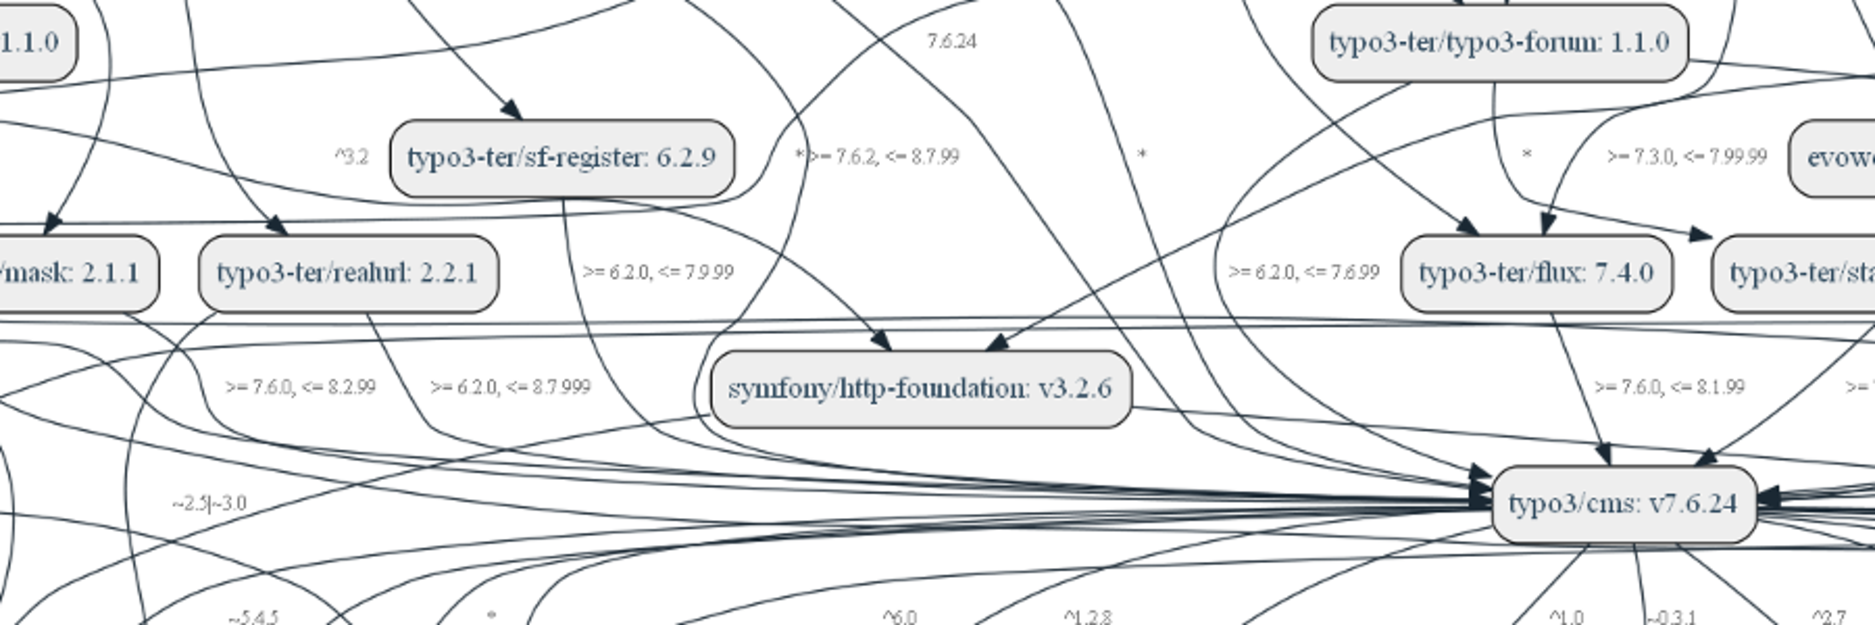
\includegraphics[
    width=\textwidth,
    height=\textheight,
    keepaspectratio
  ]{resources/dependency-graph.pdf}
  \caption{Gerichteter Graph für Abhängigkeiten}
  \label{dependency-graph}
\end{figure}

In Abbildung~\ref{dependency-graph} wurden die Abhängigkeiten der beiden Projekte in gerichtet Graphen transformiert. Dafür wurde eine PHP-Bibliothek ``clue/graph-composer'' verwendet. 

Auffällig bei beiden Projekten sind zentrale Knoten, also Abhängigkeiten die von vielen anderen Abhängigkeiten genutzt werden oder diese nutzen. Des weiteren könnten Gruppen von Abhängigkeiten ausgemacht werden. Solche Gruppen können ein eigenes, größtenteils abgrenzbares Abhängigkeitsnetz spannen. Damit dies möglich ist, müssten die Abhängigkeiten entsprechend gewichtet angeordnet sein. Im Falle des Graph-Composer-Werkzeuges erscheint dies nur mangelhaft zu gelingen. 

Abschließend sind in der Individualsoftware noch eine Reihe an unerwarteten Blattknoten erkennbar. Diese deuten auf schlecht gepflegte Abhängigkeiten hin. Unzureichende gepflegte Abhängigkeiten entstehen in der Regel, wenn die betroffenen Module nur im Gesamtkontext geprüft werden. Dadurch sind für diese Module, implizit Abhängigkeiten verfügbar, die sonst nicht nicht bereitgestellt werden könnten.

\paragraph{Kreisdiagramm}

\begin{figure}[htbp]
  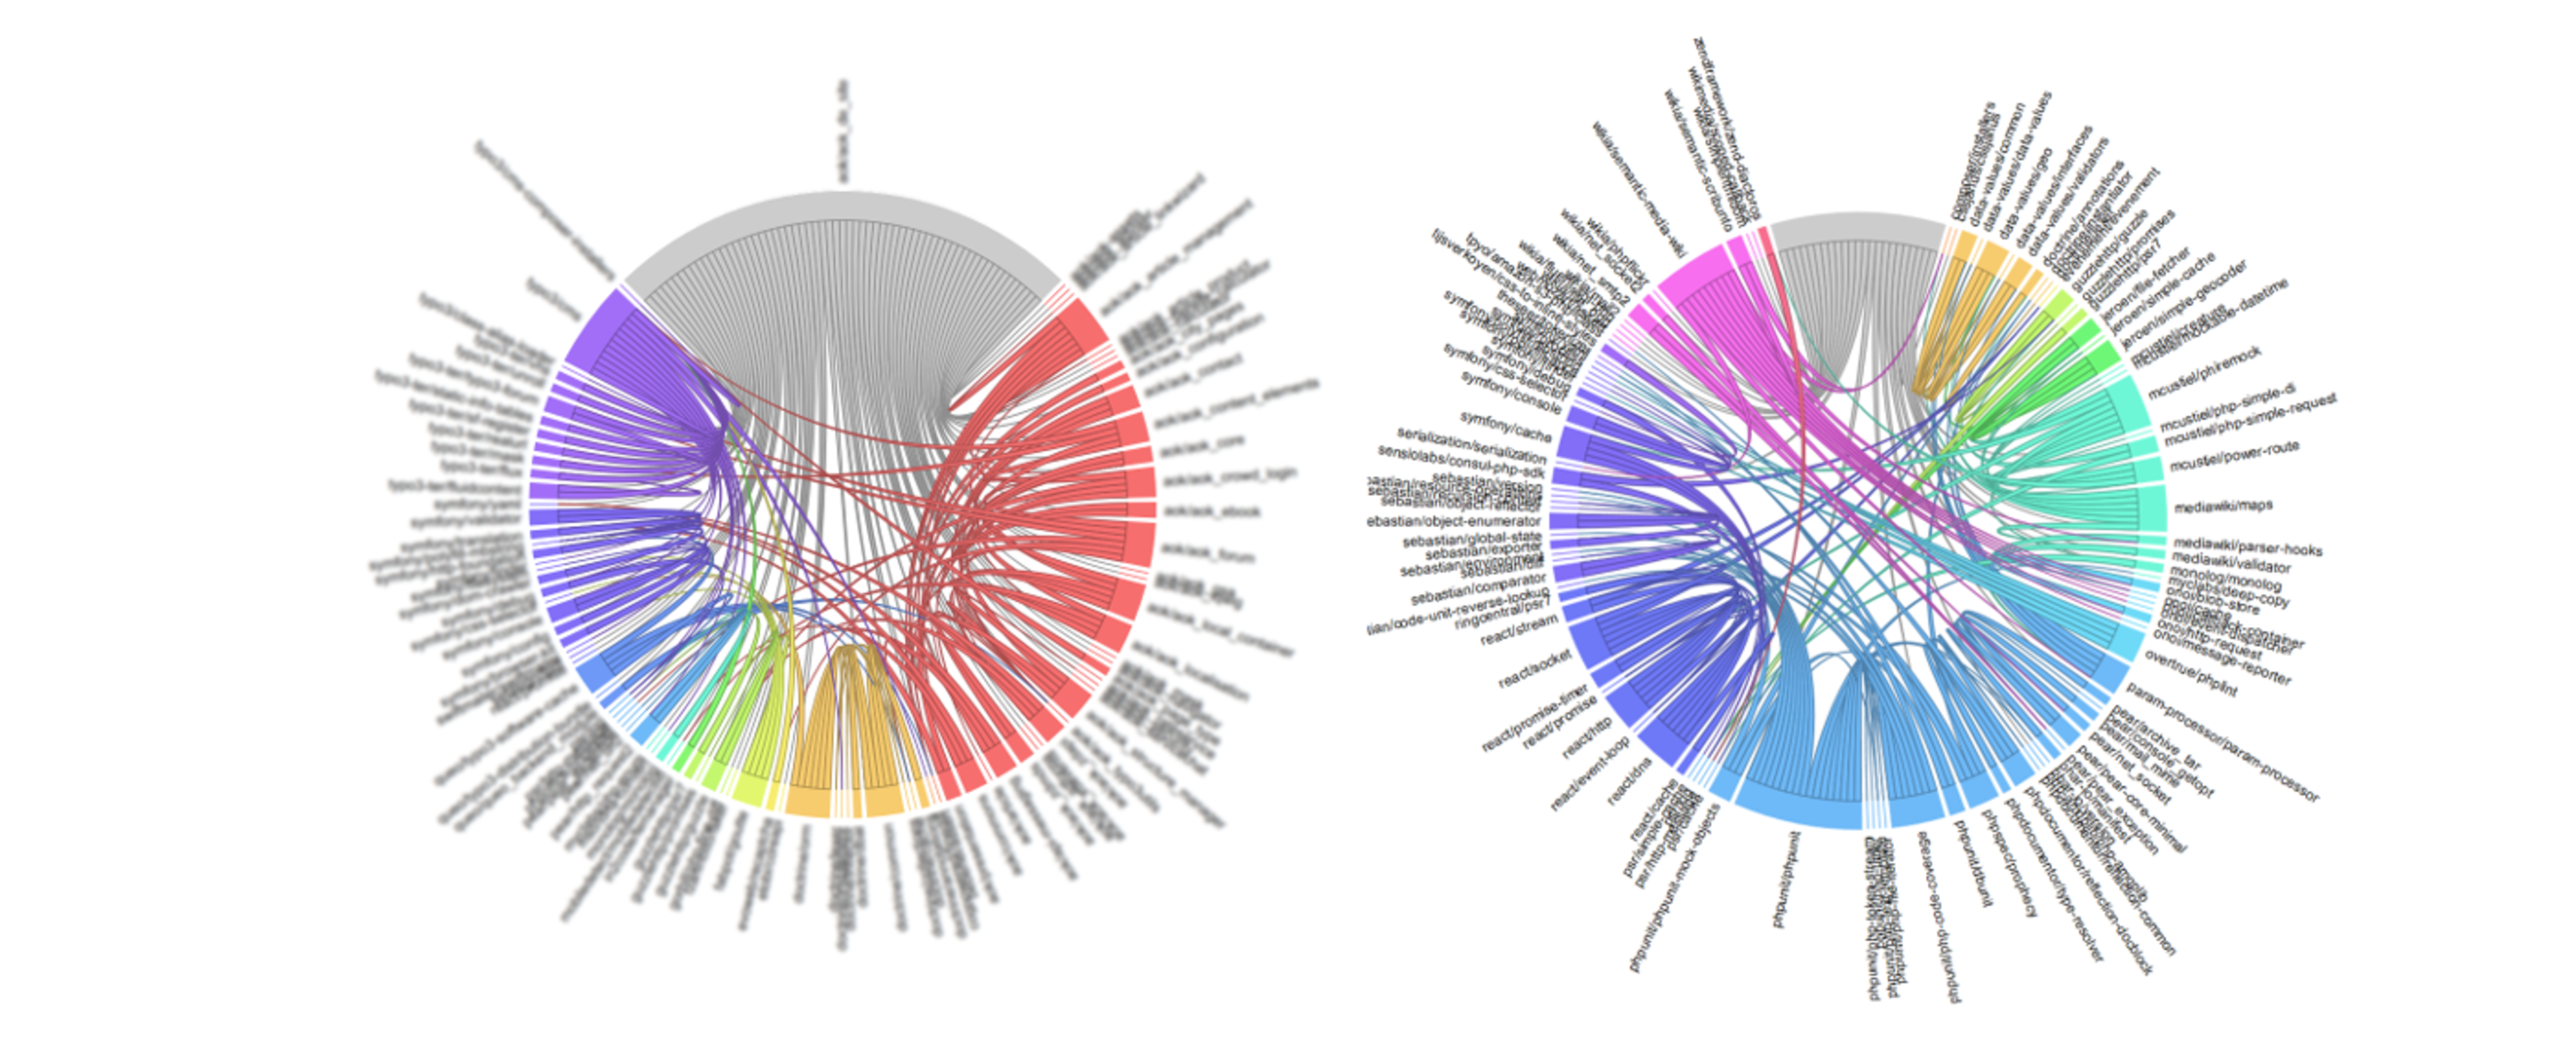
\includegraphics[
    width=\textwidth,
    height=\textheight,
    keepaspectratio
  ]{resources/circle-plot-dependencies.pdf}
  \caption{Kreisdiagramme für Abhängigkeiten}
  \label{dependency-circle-plot}
\end{figure}

In Abbildung~\ref{dependency-circle-plot} werden zwei Kreisdiagramme verwendet um die Abhängigkeitszu- und abflüsse zu verdeutlichen. Das linke Diagramm stellt die Abhängigkeiten einer mittel großen Individualsoftware für ein Content-Management-System dar. Das rechte Diagramm visualisiert die Abhängigkeiten der . Die Wahl des Kreisdiagramms ergibt sich durch seine Eignung gruppierte Ab- und Zuströme zu visualisieren\footcite{visualizing-graph-data}. 

Als Basis für die beiden Diagramme wurden die im Versionsverwaltungssystem gesichert Dateien der Packetverwaltung verwendet. Das beschreibende Format ist eine DSL von Composer\footcite{composer-json} und wird primär für PHP-Projekte verwendet. Die Ansicht wurde mit Hilfe eines JavaScript-Werkzeuges ``Dependency Wheel''\footcite{composer-dependency-wheel} erstellt.

Die grauen Abhängigkeitsteile stellen direkte Abhängigkeiten des Projektes dar, während die farbigen Stränge die Verbindungen der Abhängigkeiten visualisieren.

In der Darstellung der Individualsoftware, sind die roten Stränge interne Abhängigkeiten. Für Wikia sind Abhängigkeiten der eigenen Entwicklung Lila.

Beide Diagramme vermitteln einen guten Eindruck zur Fülle der Abhängigkeiten und eine Überblick darüber, wie viele Fremdabhängigkeiten im Projekt verwendet werden. Darüber hinaus sind allerdings nur schwer Informationen aus den sichtbaren Daten zu gewinnen. Zentrale Abhängigkeiten und Knoten lassen sich kaum ausmachen.

\paragraph{Blasendiagramm}

\begin{figure}[htbp]
  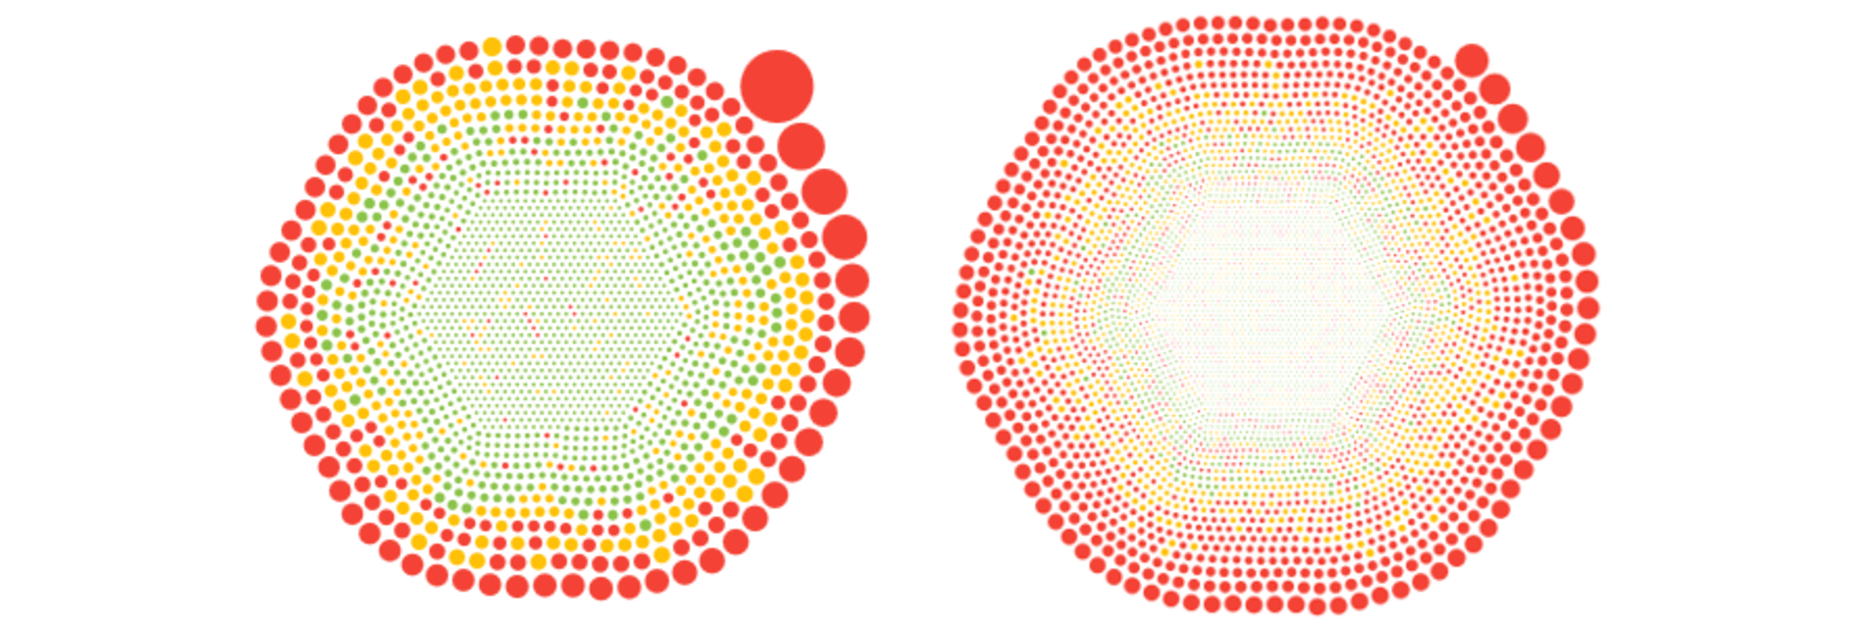
\includegraphics[
    width=\textwidth,
    height=\textheight,
    keepaspectratio
  ]{resources/bubble-complexity-chart.pdf}
  \caption{Blasendiagramm für Cyclomatische-Komplexität}
  \label{bubble-complexity}
\end{figure}

Blasendiagramme eigenen sich besonders für die relative Darstellung von Werten. Oftmals werden die Blasen zusätzlich an den Achsen eines Graphen dargestellt. Im dargestellten Beispiel wurden die Blasen sortiert aufgereiht. Jede Blase steht im Beispiel für eine Klasse und die Größe der Blase ist der Wert ihrer Cyclomatischen-Komplexität. Die Farbe der Klasse stellt einen Index für ihre Wartbarkeit zusammen. Die Darstellung ist eine Zusammenfassung der PHPMetrics-Bibliothek. 
Die Darstellung vermittelt relativ einfach die Menge und Stärke von Komplexität und potentiellen Wartungsschwierigkeiten.


\subsection{Automatisierte Systembereitstellung}

Um Feature-Branches technisch zu unterstützen, müssen Tests und Metriken für jeden Feature-Branch ausgeführt werden. Damit dies automatisiert möglich ist, müssen die zugehörigen Testsysteme automatisch zur Verfügung gestellt werden. Somit ist eine automatisierte Systembereitstellung notwendig.

Die automatische Bereitstellung ist prinzipiell sowohl mit Virtualisierung als auch mit einem Containersystem möglich. Auch eine entsprechende verwaltet Gruppe an Hardwaresystemen ist möglich, ist allerdings in den meisten Situation deutlich unwirtschaftlicher sein, als die virtuellen Lösungen.

Die Entscheidung für eine Virtualisierungs- oder Containerlösung sollte von Fall zu Fall entscheiden werden. Die schlankere und damit Resourcen schonendere Lösung ist die Verwendung von Containern. Mit ihnen können problemlos einzelne Testsysteme oder komplexere Service und Systemverbunde erstellt und verwaltet werden. Die Verwendung von Container ist nicht mehr möglich, wenn unterschiedliche Betriebs- oder Hardwaresysteme benötigt werden.

Unabhängig von der verwendeten Lösungen müssen die Systeme in einen definierten Zustand geführt werden. Dieser Vorgang kann einen größeren Zeitraum in Anspruch nehmen und benötigt entsprechend Resourcen. Um diesen Zeitraum zu verringern sollten anhand des Konfigurationsmanagements Systeme vorbereitet und in gepackter Form abgelegt werden. Bei den meisten Lösungen wird diese Form ``Image'' genannt. Wie bereits für ``Artefakt-Repositories'' angesprochen, sollten diese Images nachvollziehbar benannt und abgelegt werden. Es sollte möglich sein eine Verbindung zur jeweiligen System-Konfiguration herzustellen. Bestenfalls ist die System-Konfiguration in einer Versionsverwaltung abgelegt und die entsprechende Version kann ebenfalls zur Referenzierung des System-Images verwendet werden. Im Rahmen des automatisieren Bereitstellungsprozesses wäre es auch sinnvoll die verwendet Systemkonfiguration in der Entsprechenden System-Übersicht aus Kapitel~\ref{subsubsec:configuration-system-overview} zu aktualisieren.

\section{Best Practices in der Softwareentwicklung}

Feature-Branches beheben Hindernisse, die beim Zusammenführen von Änderungen auftreten nicht. Sie helfen lediglich diese Hindernisse in gezielter und geordneter Weise anzugehen. Daher sind Entwickler auch mit Features-Branches darauf angewiesen Entwicklungsmuster anzuwenden und sich mit der Softwarearchitektur der Anwendung auseinanderzusetzen.

Viele dieser Entwicklungsmuster und -verfahren werden unter dem Begriff ``Best Practices'' geführt. Sie unterstützen Entwickler in Entwurfsentscheidungen und geben Rahmen für Standards in der Softwareentwicklung. Viele der Best-Practices zielen zudem auf Verbesserungen für Wartbarkeit, Robustheit und allgemeine geringere Umsetzungsaufwände.

\subsection{Modularisierung von Software}

Viele Probleme bei Continuous-Integration und Feature-Branches entstehen bei komplizierten Merge-Verfahren. Viele komplizierte Merge-Schritte begründen sich häufig durch einen zu hohen Kopplungsgrad der Software. Wenn Komponenten stark gekoppelt sind, ist es oft notwendig mit mehreren Entwicklern in gleichen Code-Abschnitten zu interagieren. Wird eine Software von Beginn an lose gekoppelt entwickelt, ergeben sich oft deutlich weniger Abhängigkeiten und komplizierte Merge-Schritte werden vermieden.

Die lose Kopplung einer Software kann, durch das Einhalten der Prinzipien zur Modularisierung\footcite{2012-barth-modularisation}, erreicht werden. 

\paragraph{Information Hiding} ist ein von Parnas\footcite{1972-parnas} geprägter Begriff. Als Basis für die Modularisierung und Dekomposition von Software wird drei Schritten gefolgt:
\begin{itemize}
\item Ermittle alle Entwurfsentscheidungen, welche sich potentiell ändern werden.
\item Erstelle pro Entwurfsentscheidung ein Modul, die Entwurfsentscheidung wird ``Geheimnis des Moduls'' genannt.
\item Die Schnittstelle zum Modul sollte robust genug sein, um bei einer Änderung des Geheimnisses nicht verändert zu werden.
\end{itemize}
Durch die Einhaltung der Prinzipien, werden mögliche Änderungen auf ein Modul beschränkt und damit die Auswirkungen begrenzt.
\paragraph{Separation of Concerns} ist ein Basisprinzip moderner Softwareentwicklung. Während Information-Hiding auf einer niedrigen Modulebene ansetzt, versucht die ``Aufteilung nach Anliegen'' höher anzusetzen. Die Teile eines Moduls sollen nach möglich Anliegen  mit möglich wenig Überlappungen eingeteilt werden. 
\paragraph{Low Coupling Cohesion} beschreibt das Verbindungs- und Kommunikationsverhalten der Module. Es wird eine hohe Kohäsion innerhalb eines Moduls angestrebt und eine geringe zu anderen Modulen.

Werden die Prinzipien befolgt, ergeben sich Vorteile für die Wartbarkeit, Wiederverwendbarkeit und Robustheit der Anwendung. Die Konzentrierten Verbindungen sorgen zudem für eine geringere Schnittmenge von Änderungen durch Entwickler.

Eine modernere Form der Modularisierung sind die ``serviceorientierten Architekturen''. Diese beschreiben Anwendungsszenarien in verschiedenen Granularität. Die Kapselung in Services ermöglichen die Komposition und Orchestrierung von komplexen Vorgängen. Der serviceorientierte Ansatz nutzt die Prinzipien der Modularisierung und bietet die Vorteile unter neuem Namen an.

\subsection{Fortgeschrittene Nutzung von Versionsverwaltung}

Wie auch mit jeder anderen Versionsverwaltung, so ist es auch beim Arbeiten mit Git essentiell, seine Arbeit zu strukturieren. Wird Git lediglich als bequeme Variante für eine regelmäßige Sicherung des Arbeitsstandes genutzt, dann entsteht sehr schnell eine schwer zu lesende, an Bedeutung mangelnde Versionshistorie. Wichtig ist es die getätigte Arbeit in semantisch zusammenhängenden, möglichst kleine und prägnanten Commits zu gliedern. Ein Commit sollte immer nur eine Änderung zusammenfassen. Dadurch ist es möglich feingranulare Commit-Nachrichten zu verfassen.
Zusammen mit nachvollziehbaren und klaren Commit-Nachrichten, entsteht so eine gut leserliche und die Dokumentation unterstützende Versionshistorie.\footcite[vgl.][Kap. Making only one change per commit]{git-essentials-2017}

\footcite[Writing commit messages before starting to code][]{git-essentials-2017}

Including the whole change in one commit

Describing the change, not what have you done

\subsection{Testgetriebene Entwicklung}
\label{test-driven-development}

Testgetriebene Entwicklung, oder auch Test-Driven-Development(TDD) wurde bereits von Kent Beck 1999 als ``test-first''-Ansatz propagiert. Seitdem hat dieses Vorgehen viele Anhänger gewonnen. Es fordert ein Umdenken beim Entwickler. Zuerst muss das Ergebnis einer Änderung oder einer Neuerung bekannt sein und erst danach kann der umsetzende Code entwickelt werden\footcite[vgl.][Kap. Understanding TDD]{tdd-java}. Die Umkehrung des Zeitpunktes, wann die Tests verfasst werden, fördert die Qualität der Entwicklung. Es werden die Anzahl der auftretenden Fehler reduziert, entkoppelte Strukturen gefördert und die Anzahl der nachträglich auftretenden Fehler deutlich gemindert\footcite[vgl.][]{tdd-ci-effectivness}.
Insbesondere im Continuous-Integration-Bereich ist TDD als Continuous-Testing sinnvoll, da nur kontinuierlich getesteter Code auch kontinuierlich zuverlässig integriert werden kann.

Die Art und Weise der Anwendung von TDD kann stark variieren. Daher wird eine stark iterative Variante des Schreibens von Tests angestrebt. Das ``Red Green Refactoring''\footcite[vgl.][Kap. 
Red-Green-Refactor
]{tdd-java} fordert immer nur minimale Anpassungen vorzunehmen, bis der Test vollständig ist. Nach jeder Anpassung, die den Test fehlschlagen lässt, muss die getestete Implementierung so angepasst werden, dass der Test erfolgreich verläuft. Ist der Test vollständig muss abschließend die Implementierung einem Refactoring unterzogen werden. Basierend auf der begrenzten gedanklichen Kapazität eines Entwicklers, soll so immer nur ein Gesichtspunkt der Entwicklung betrachtet werden. Zuerst soll das korrekte Verhalten der Software sichergestellt werden. Danach ist die korrekte Struktur der Software herzustellen. Die Dualität der Betrachtung und der minimal inkrementelle Ansatz sollen ein hoch qualitatives Resultat ergeben.

Über die Lehrmethoden von TDD sind bekannte Verbindungen von Anforderungsmanagement und Testfallerstellung, wieder in den Fokus gerückt. Unter der Bezeichnung ``Behaviour-Driven-Development''\footcite{bdd-north} entstand ein Verfahren zur Verbindung beider Bereiche. Mittels einer der Umgangssprache nahen DSL wird versucht eine leserliche Dokumentation zu erstellen. Nutzerszenarien werden in einer Gegeben-Wenn-Dann-Notation\footcite{fowler-gwt} verfasst und können durch die strukturierte Notation direkt mit Test-Code verknüpft werden. Damit wird angestrebt die Barrieren zwischen Projektteilnehmern ohne Programmierkenntnissen, Testern und Entwicklern zu verringern.

\subsection{Verwendung von Monorepo-Repositories}

Im Abschnitt~\ref{subsubsec:illustrate-dependencies}~``\nameref{subsubsec:illustrate-dependencies}'', konnten gut Abhängigkeitsgruppierungen erkannt werden. Gerade bei Abhängigkeitskonstrukten innerhalb einer Organisation, werden häufig Änderungen parallel in mehreren Abhängigkeiten vorgenommen. Gerade wenn sich diese Abhängigkeiten gegenseitig bedingen, kann es zu einem erhöhten Aufwand kommen. Damit ein gemeinsamer Stand erreicht wird, müssen häufig mehrere Teile des Projektes aktualisiert werden. Gerade wenn ein experimentelles Feature auf mehreren zusammenhängenden Feature-Branches getestet werden muss, entsteht ein deutlich erhöhter Aufwand.

Eine Variante diese Aufwände zu reduzieren und Tests, sowie Auslieferung von Software für ein Paket von Abhängigkeiten zu optimieren, sind Monorepos. Monorepos verwenden, im Kontrast zu regulären Praktiken, ein Repository für mehrere Abhängigkeiten\footcite{trunkbaseddevelopment-monorepo}. Dieses Vorgehen hat den direkten Vorteil, dass Abhängigkeiten nicht miteinander verlinkt werden müssen. Abhängigkeiten sind durch das gemeinsam geteilte Repository automatisch verbunden. Zudem können gemeinsam verwendete Werkzeug einfach gleichgeschaltet und die gemeinsame Verwendung begünstigt werden.

Die Verwendung eines Monorepos vereinfacht zwar die Abhängigkeitsverwaltung, birgt allerdings Schwierigkeiten für größere Repositories. Während in Repositories getrennte Abhängigkeiten, auch die Commits logisch und physisch getrennt sind, fällt diese Barriere in Monorepos. Es müssen daher zusätzliche Mechanismen für die Übersicht geschaffen werden.

Ein weiterer Punkt ist die Performance. Abhängig vom gewählten Versionsverwaltungssystem, können gerade mit Git hier Probleme auftreten. Da Git immer die vollständige Historie bereit hält, sind Performance-Probleme spürbar\footcite{atlassian-monorepo-git}. In zentralen Systemen wie SVN können für Monorepos gezielte Teilebereiche des Repos verwendet werden. 
In jedem Versionsverwaltungssystem ist hingegen die erhöhte Commit-Frequenz spürbar. Merges treten deutlich häufiger auf, zusätzliche manuelle Eingriffe sind teilweise notwendig.

Trotz der Schwierigkeiten nutzen große Unternehmen wie Google, Facebook und Twitter sehr große Monorepos. Für alle drei Unternehmen ist die Verwendung von Monorepos allerdings mit großem Aufwand verbunden. Google entwickelte eine eigene Versionsverwaltung, Facebook investiert in Mercurial und Twitter verwendet eine speziell angepasste Git-Variante\footcite{monorepos-wild}.
Bei entsprechender Größe des Projektes, ist allerdings auch für kleinere Unternehmen die Verwendung von Monorepos nützlich\footcite{hackernoon-positive-monorepo}.

\section{Prototyp zur Feature-Branch-Visualisierung}

Mit wachsender Beliebtheit von Feature-Branches, erweiterten auch die Anbieter für Continuous-Integration-Lösungen ihr Angebot. Viele Anbieter stellen umfangreiche Angebote für Continuous-Deployment bereit. Oftmals sind auch zusätzliche Optionen für Feature-Branches enthalten. Wie im Git-Workflow vorgestellt, werden diese Feature-Branches durch einen manuellen Merge-Befehl auf einem Release-Branch akkumuliert. Auf diese Weise werden kontinuierlich, wenn auch verzögert, die einzelnen Feature-Branches mit einander zusammengeführt. Das späte Feedback zum Zeitpunkt der Zusammenführung, kann zu Problemen und zur Verzögerungen beim Release führen. Eine direkte Alternative ist es, die jeweiligen Feature-Branches direkt zum Zeitpunkt ihrer Fertigstellung zusammenzuführen. Für jeden weiteren Feature-Branch, der zusammengeführt werden muss, ergeben sich allerdings die gleichen Problem, wie bereits zuvor.
Eine mögliche Lösung wäre es Release bereits im Vorfeld zu definieren und die dazugehörigen Branches zu verfolgen. Somit können Konflikten in Codeständen und potentielle Fehlerquellen eher erkennen. Sind alle Feature-Branches konfliktfrei, können diese automatisch zu einem Release gebündelt werden. Jeder einzelne Branch kann durch Tests und Metriken unterstützt werden. Zudem können auf diese Weise Features zurückgehalten werden, die fertig gestellt wurden, aber aus politischen Gründen noch nicht Teil des Releases sein dürfen. 
Die Behebung von Merge-Konflikten bedeutet, dass einer der beiden vom Konflikt betroffenen Branches, Teile des Codes des anderen Branches, mit aufnehmen muss. Daher ist es möglich, dass auch mit der Verwendung von Feature-Branches, das gezielte zurückhalten von Features, schwierig bleibt. Daher können dieses beiden Branches nicht ohne ein Feature-Toggle unabhängig von einander veröffentlicht werden.

Der Prototyp soll somit die folgenden Punkte unterstützen:
\begin{itemize}
\item Gruppierung von Feature-Branches zu Releases
\item Darstellung der Untermenge an Branches, welche bereits zu einem Release kombiniert werden können
\item Darstellung der Testergebnisse, Testabdeckung und Code-Qualitätsmetriken
\item Bereitstellung einer API um Testergebnisse und Metriken mit einem Continuous-Integration-System zu synchronisieren
\end{itemize}

\subsection{Anforderungen}

Ziel des Prototyps ist es Release-Informationen zu einem Projekt anzuzeigen. Daher müssen Projekte angelegt und bearbeitet werden. Zudem müssen die zugehörigen Repository-Informationen ausgelesen werden. Weiter sollten Abhängigkeiten des Projektes ausgelesen und ausgewertet werden. 

Um einzuordnen, welche Änderungen zu einem Release gehören, müssen diese Änderungen definiert werden. Im Fall von Feature-Branches müssen die Feature-Branches deklariert werden, welche Teil des Releases werden. Damit ein Release aussagekräftig deklariert wird, sollten zudem Feature-Branches innerhalb der Abhängigkeiten deklariert werden.

Ist das Release definiert, sollen eine Reihe an Fragen einfach zu beantworten sein. 
\begin{itemize}
\item Können alle Feature-Branches zusammengeführt werden?
\item Welche Branches würde einen Konflikt mit welchem anderen Branch auslösen?
\item Wie sieht die derzeit minimal release-fähige Untermenge an Feature-Branches aus?
\item Welche Branches wurden erfolgreich getestet?
\item Wie verhalten sich die Metriken der Feature-Branches untereinander und zum Haupt-Branch?
\end{itemize}

Des Weiteren sollte die Anwendung an einen bestehenden Continuous-Prozess möglich sein. Es sollte daher eine REST-API bereit gestellt werden. Die API soll primär die Daten für Metriken und Testergebnisse entgegennehmen.

\subsection{Nutzungsszenarien (Use-Cases)}

Aus den Anforderungen ergeben sich einige Nutzungsszenarien. Es soll keine vollständige Projektspezifikation für den Prototypen erstellt werden, daher werden die Nutzungsszenarien nur angerissen. 

\paragraph{Projekt registrieren}
Um die Projekte zu analysieren, müssen sie angelegt werden. Im optimal Fall geschieht dies durch die Angabe eines Repositories. Aus diesem Repository können, anhand der Beschreibungsdatei der verwendeten Packetverwaltung, die weiteren Informationen gewonnen werden.

\paragraph{Branches auflisten}
Um die Feature-Branches für ein Release zu selektieren, müssen alle verfügbaren Branches des Projektes dargestellt werden. 

\paragraph{Release erstellen}
Die Release-Erstellung erfolgt durch die Wahl eines Namens und der Selektion der gewünschten Branches. Der Release wird dem Projekt zugeordnet und kann über das Projekt angezeigt werden.

\paragraph{Branch-Details darstellen}
Um einen Branch zu bewerten, müssen Tests und Metriken für den Branch ausgeführt werden. Die Ausführung und die Sammlung der Daten werden außerhalb des Tools durchgeführt, daher werden diese Daten über eine API zugeführt.

\paragraph{Branch-Konflikte anzeigen}
Zur weiteren Bewertung der Branches müssen Merge-Konflikte zwischen den Branches ermittelt werden. Branche die einen Konflikt aufweisen, sollten in der Release-Übersicht markiert und gruppiert werden.

\paragraph{Release erstellen}
Um Wunsch wird ein Release-Branch erstellt und alle Branches, die keinen Konflikt aufweisen, werden zusammengeführt.

\subsection{Grundlagen der Umsetzung}

Da der Prototyp als Unterstützung für bestehende Werkzeuge agieren soll, bietet sich ein modernes Web-Framework an. Durch die berufliche Prägung des Autors der Masterarbeit, liegt der Fokus zudem auf PHP. Die Wahl für ein modernes und flexibles Framework fällt daher auf Symfony, welches sich durch Flexibilität und Modularität auszeichnet. Zudem existiert für Symfony eine sehr aktive Community, welche Zahlreiche Werkzeug und Hilfsbibliotheken bereit stellt. Durch Symfony ergibt sich als bevorzugte Abhängigkeitsverwaltung Composer.  

\subsection{Domainmodell}

Das betrachtet Problem betrifft sowohl Repository-Artefakte, als auch Projekt- und Release-Details. Weiter müssen Metriken und Testergebnisse protokolliert werden. Da die Erstellung von Metriken und Tests eine größere Zeitspanne benötigen können, müssen die Ergebnisse in jedem Fall persistiert werden. Ist zudem gefordert, dass der Zugriff auf das Versionsverwaltungssystem nur im Command-Line-Level erfolgen darf und nicht über die Webschnittstelle, ist auch hier die Notwendigkeit der Persistierung gegeben.

\begin{figure}[htbp]
  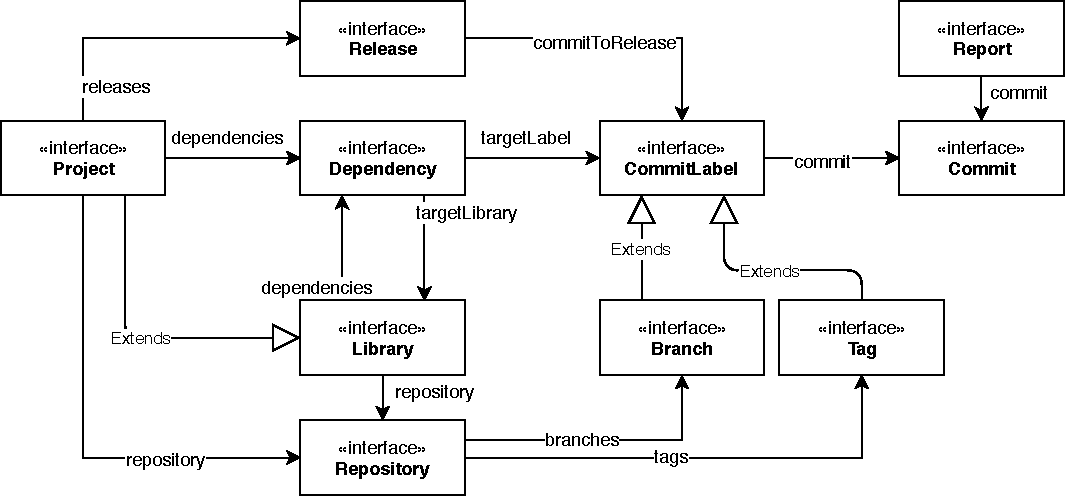
\includegraphics[
    width=\textwidth,
    height=\textheight,
    keepaspectratio
  ]{resources/ReleaseWardenClassChart.pdf}
  \caption{Klassendiagramm für Domainmodell}
  \label{class-chart-release-warden}
\end{figure}

In Abbildung~\ref{class-chart-release-warden} wird das Domainmodell in einem UML-Klassendiagramm dargestellt. Das Domainmodell beschreibt ein betrachtetes Projekt(Project) mit seinen Abhängigkeiten(Dependency) und den Releases für das Projekt. 
Um die Abhängigkeiten abzubilden und die verfügbaren Feature-Branches für ein Release zu selektieren, werden somit auch die Repositories und ihre Branches und Tags benötigt.

\subsection{Umsetzung der Nutzerszenarien}

\paragraph{Projekt registrieren}

\paragraph{Branches auflisten}

\paragraph{Release erstellen}

\paragraph{Branch-Details anzeigen}

\paragraph{Branch-Konflikte anzeigen}

\paragraph{Release erstellen}

Beschreibung von PHPMetrics


\section{Motivation, Disziplin und Verantwortung - Faktor Mensch}
\label{sec:human-fail}
Die vorangegangene Kapitel beschäftigen sich größtenteils mit Methodiken und Hilfsmitteln. Die Motivation dieser Methodiken und Hilfsmittel begrenzt sich unter anderem auf Wartbarkeit, Robustheit und Skalierbarkeit von Software. Dabei wird die Motivation für die Entwicklung, genauer für den Entwickler, weitestgehend ausgelassen.

Gerade in Anbetracht der Zeit, die viele der Methodiken bereits bekannt sind, ist es hilfreich einen weiteren Aspekt hinzuziehen. Dieser Aspekt soll den psychischen Teil der Einführung einer neuen Methodik beleuchten.

\subsection{Motivation}

Motivation kann durch drei Bereiche getragen werden\footcite[vgl.][]{codingame-drive}\footcite[vgl.][Kap. Autonomie ff.]{pink-drive}:
\begin{itemize}
\item Autonomie - die Möglichkeit sich selbst zu organisieren. Autonomie soll die eigenen Fähigkeiten möglichst voll zu nutzen.
\item Können - die Möglichkeit sich weiterzuentwickeln und Neues zu entdecken.
\item Bestimmung - die Möglichkeit an etwas mit Bedeutung mitzuwirken.
\end{itemize}

Die Einteilung ist eine Zusammenfassung mehrere einzelner Theorien und in manchen Teilen populärwissenschaftlich\footcite[vgl.][]{drive-scholarly-review}. Basierend auf den drei Bereichen, können die Methodiken besser argumentiert und die generelle Bereitschaft zur Einführung gestärkt werden. Generell sollte jeder Teilnehmer einer Methodik sich darin wiederfinden. Methodiken die sich nicht im Alltag des Entwicklungsteams wiederfinden, werden auf lange Sicht verschwinden oder zur Belastung.

\subsection{Disziplin}

Viele eingeführte Hilfsmittel, Methodiken oder Ideen verschwinden wieder. Oftmals fehlen Träger und Fürsprecher. Häufig fehlt es aber auch an Disziplin. Entscheidend ist die Einsicht zur Selbstdisziplin. Viele agile Methodiken basieren auf Selbstorganisation und Eigenverantwortung\footcite[vgl.][]{codingame-agile-failed}. Viele der Methodiken basieren auf einem Entwickler, der bereit ist stetig zu wachsen und an sich zu arbeiten.
Disziplin greift nach der Motivation. Nach der Einführung einer neuen Methodik, benötigt es oft Disziplin diese aktiv zu nutzen\footcite[vgl.][]{screw-motivation}. Es benötigt konstante Arbeit und Reflexion zur Nutzung und Erhaltung einer neuen Methodik.

Oftmals ist eine neue Methodik damit verbunden, alte Verhaltensweisen abzulegen.
Gelernte Verhaltensweise lassen sich oft eine Folge von drei Punkten gliedern.
\begin{itemize}
\item Auslöser - die Situation, welche eine Gewohnheit auslöst oder diese einleitet.
\item Verhalten - der Ablauf oder das Verhalten, welches die Gewohnheit darstellt.
\item Nutzen - der Nutzen, welchen das Verhalten erzeugt.
\end{itemize}
Die Hemmschwelle zur Einführung einer neuen Methodik sollte möglichst gering gehalten werden. Dazu bietet es sich an die Methodik an bereits existierende Mechanismen zu knüpfen. Zudem sollte der Aufwand zur Nutzung sehr gering sein und der Nutzen durch eine Rückkopplung spürbar\footcite[vgl.][]{steps-of-habit}.

\subsection{Verantwortung}

Auch eine Methodik die durch Träger und Fürsprecher eingeführt wird, sollte in der Verantwortung des ganzen Entwicklungsteam liegen. Die Einhaltung der Methodik sollte jeden, der sie missachtet, in die Verantwortung ziehen.
Wie auch in vielen agilen Methodiken, ist eine gemeinsame Fürsprache, ein gemeinsames ``Commitment'' notwendig. Ein gemeinsames Commitment sollte, wenn möglich, durch technische Hilfsmittel unterstütze werden. Für viele gemeinsame Regeln existieren automatisierte Prüfungen oder Integrationen für die Entwicklungsumgebung und den automatisierten Software-Erstellungsprozess.
Auch der Review-Prozess für Softwareänderungen kann hierbei unterstützen. Entwickler sollten sich stets gegenseitig auf die Missachtung von Coding-Guidelines und Entwicklungsmustern hinweisen.

\subsection{Faktor Mensch}

Die Erstellung von Software verlangt eine breite Palette an Fähigkeiten. Zudem fehlen in der Softwareerstellung viele der standardisierten Vorgehensweisen der Ingenieursdisziplinen. Häufig werden kreative und pragmatische Lösungen benötigt.

\blockquote {discipline, the most lacking virtue in creative people (like programmers)}\footcite[][S.167]{git-essentials-2017}
\vspace{1em}\\
Die fehlenden Standards und Notwendigkeit für kreativen Lösungen von Entwicklern, sind ein zu respektierendes Risiko in der Softwareentwicklung. Fordernde und anspruchsvolle Methodiken sind nicht für alle Softwareentwickler geeignet. Laufende Projekte und bestehende Belastungen sind bei der Einführung neuer Methodiken stets zu beachten. Die Einführung neuer Methodiken in bereits belastete oder scheiternde Projekte führen oft zu schlimmeren Ergebnissen.

Neue Methodiken sollten stets mit dem nötigen Raum eingeführt werden. Zudem sollte eine regelmäßige Betrachtung des Verhältnisses von Aufwand und Nutzen erfolgen.


\chapter{Zusammenfassung}

während ci die last der integration auf den Schultern aller aushandelt, verlagert fb die integration auf den schultern des ``konfliktverursachers'' somit wird eine kommunikation gefördert, allerdings ohne blockierende nachteile (rote ci ampeln als anti-pattern)

unabhängig von ci und fb sollten systeme clean code ansätze nutzen um gut skalierbare, wartungsarme systeme zu erstellen

\appendix
\printbibliography[heading=bibintoc]

\end{document}